\chapter{\iftoggle{german}{Verwandte Arbeiten}{Background and Related Work}}\label{ch:related_work}

In this chapter, we discuss the task we will evaluate and the previous work related to the task.
In \autoref{sec:3D_reconstruction}, we define the 3D reconstruction tasks.
\autoref{sec:state_of_the_art} will contain state-of-the-art 3D Reconstruction techniques used with different model representations(Voxels, Mesh, Point Clouds).
We then discuss the baseline models in \autoref{subsec:pix2vox-and-pix2vox++} which will be used in \autoref{ch:evaluation}.

We will also discuss the previous contributions to indoor datasets in \autoref{sec:indoor-dataset},
what tasks each dataset supports, and some disadvantages.
Further, we discuss the available tools which support the creation of indoor dataset \autoref{subsec:tools-to-create-synthetic} on different platforms and frameworks.

We then discuss about Domain space in \autoref{sec:domain-space}, how we visualize it qualitatively and quantitatively.
We will also discuss ways to mitigate the domain gap in \autoref{sec:mitigating_domain_shift}.
This section will include traditional techniques like transfer learning or fine-tuning and mixed training.
Recent trends in Generative models to transfer the style of the real image onto synthetically generated images is also briefly discussed.

\section{3D reconstruction}\label{sec:3D_reconstruction}
The main task of this thesis is the reconstruct a furniture from RGB image.
For this purpose, we take a Deep Learning approach for 3D-Reconstruction.
3D reconstruction is converting a 2-Dimensional RGB image into an available 3D representation of the model under observation.

The training examples are of the form  $\{(x_1,y_1),(x_2,y_2) \dots(x_n,y_n)\}$ where $x_k$ are 2D images, and $y_k$ are 3D model discretized to obtain a 3D voxel grid.
3D reconstruction is a learning task which seeks $g: X \to Y$, where $X$ is 2D input space and $Y$ is 3D output space.
The task minimizes an objective function $Obj(g) = \frac{1}{N} \sum_i L(y_i, g(x_i))$, where $L$ is a loss function.

In this thesis, we consider an architecture that consists of an encoder and decoder.
~\cite{Han2021ImageBased3O} discussed that an encoder maps a 2D image into a latent space by converting pixel grid into feature vectors.
If we formulate the problem, $Enc: X \to V$, where $Enc$ is the encoder function, $X$ is the input image space, and $V$ is the latent space.
An encoder is a good mapping function if for the given set of images of same category $x = \{x_k \mid k = 1,2,\dots c\}$, the corresponding feature vectors $v = \{v_k \mid k = 1,2,\dots c\}$ are close together in given latent space $V$
irrespective of the extrinsic parameters like textures, background, camera positions,etc.

The decoder is an expansive network, which converts a feature vector from the latent space into a 3D voxel grid.
$Dec: V \to Y$, i.e. for any vector in latent space $V$, the decoder function \textbf{$Dec$} should be able to create a 3D voxel grid in $Y$.
If the images are encoded perfectly, a slight change in the feature vector will give a slight variation in the 3D voxel.

\subsection{State of the art for 3d-reconstruction}\label{sec:state_of_the_art}

3D reconstruction task is on the rise with improvements in technologies like Augmented and virtual reality.
Scene understanding becomes essential for these technologies to succeed.
As discussed in \autoref{sec:Volumetric representation}, 3D models have voxels, meshes, and point clouds as representations.
Each of the representations has been explored for reconstruction, and this section explores some approaches.

The task can either be applied to \b{a multi-view, or a single view image}.
~\cite{Kar2017, choy20163d, Yang_2019, Huang2018, Paschalidou2018RayNetLV, Xie_2019, Xie_2020},
are architectures based on multiple input images of the same images from different views to learn the underlying 3D structure.
~\cite{Kar2017, choy20163d} are architectures based on Recurrent Neural Networks (\gls{rnn}) and have the disadvantage of memory,
long-term dependencies, and long inference time.
~\cite{Yang_2019, Huang2018, Paschalidou2018RayNetLV} explore different ways of pooling(attentional, max, and average pooling, respectively)
to aggregate the feature vectors from different views.
The pooling method tends to capture only partial information with loss in detail.

For single-view reconstruction, we have architectures like~\cite{Wu2017,z-gan, Yang2019, Wu2018, popov2020corenet}.
~\cite{Wu2017} predict the 3D structure by estimating 2.5D properties like surface normals, segmentation, and depths.
~\cite{Wu2018} is an extension of MarrNet, which proposes a network to preserve the naturalness of the surface.
Inspired by generative models~\cite{Goodfellow2014,Kingma2014}, many 3D reconstruction architectures were published~\cite{z-gan, Yang2019,Wu2016,Lunz2020InverseGG}.
Both~\cite{Xie_2019, Xie_2020} also can predict 3D structure from a single view image.

Many new architectures have also been proposed to overcome the memory issues caused by 3D voxels~\cite{tatarchenko2017octree,Roth2018,Mescheder2019OccupancyNL,Gkioxari2019MeshR, wang2018pixel2mesh,groueix2018atlasnet,pan2019deep}.
These are approaches that are based out of oct-tree, meshes, occupancy of a voxel.
Occupancy networks are an implicit way of representing 3D surfaces as decision boundaries using the network as a deep learning classifier.
For mesh-based reconstruction, a template mesh such as an ellipsoid is deformed to get the structure of the 3D model.
For the Oct-tree-based reconstruction, as the name suggests, instead of 3D voxels, the models are discretized in Oct-Tree representation.
Oct-tree can further make the process memory and compute efficient, providing higher resolution than 3D voxel representation.

Supervision is another factor to consider for 3D reconstruction tasks.
There are methods based on \b{3D-Supervision or 2D-Supervision}.
~\cite{Xie_2019,Xie_2020,Wu2017,groueix2018atlasnet,pan2019deep, chen2019learning} are few of the 3D-supervision based architecture.
For all these architectures, it is necessary to either have the 3D voxel grid or 3D mesh for supervised training.
For models described in~\cite{Lunz2020InverseGG,henderson2019learning},the 3D reconstruction only needs 2D supervision like a silhouette.
One might argue that for 3D supervision, we need a large number of 3D models designed and created by professional artists
With the advent of Virtual and Augmented realities, 3D models available to the public is increasing exponentially, which might resolve the issue.

\subsection{Pix2Vox and Pix2Vox++}\label{subsec:pix2vox-and-pix2vox++}
The architecture of Pix2Vox~\cite{Xie_2019} is as shown in \autoref{fig:architectures}(a).
The network consists of 4 modules: Encoder, Decoder, Merger, and Refiner.
Merger plays a significant part when it comes to the multi-view reconstruction of 3d objects.
As we focus on single-view 3d reconstruction, the merger module will not influence the output significantly.
As an encoder, Pix2Vox has utilized \gls{vgg}16 network~\cite{simonyan2015deep} pre-trained on ImageNet~\cite{Deng2009ImageNetAL}.
The decoder is an expansive network that converts 2D embeddings to a 3D voxel grid.
The refiner is an auto-encoder that takes the 3D output from the merger and produces a more refined final output.
A second paper based on Pix2Vox was titled Pix2Vox++~\cite{Xie_2020}.
The extended work replaces \gls{vgg} encoder~\cite{simonyan2015deep} with \gls{resnet}~\cite{He2016DeepRL}.

\begin{figure}[!ht]
    \centering
    \subfloat[][]{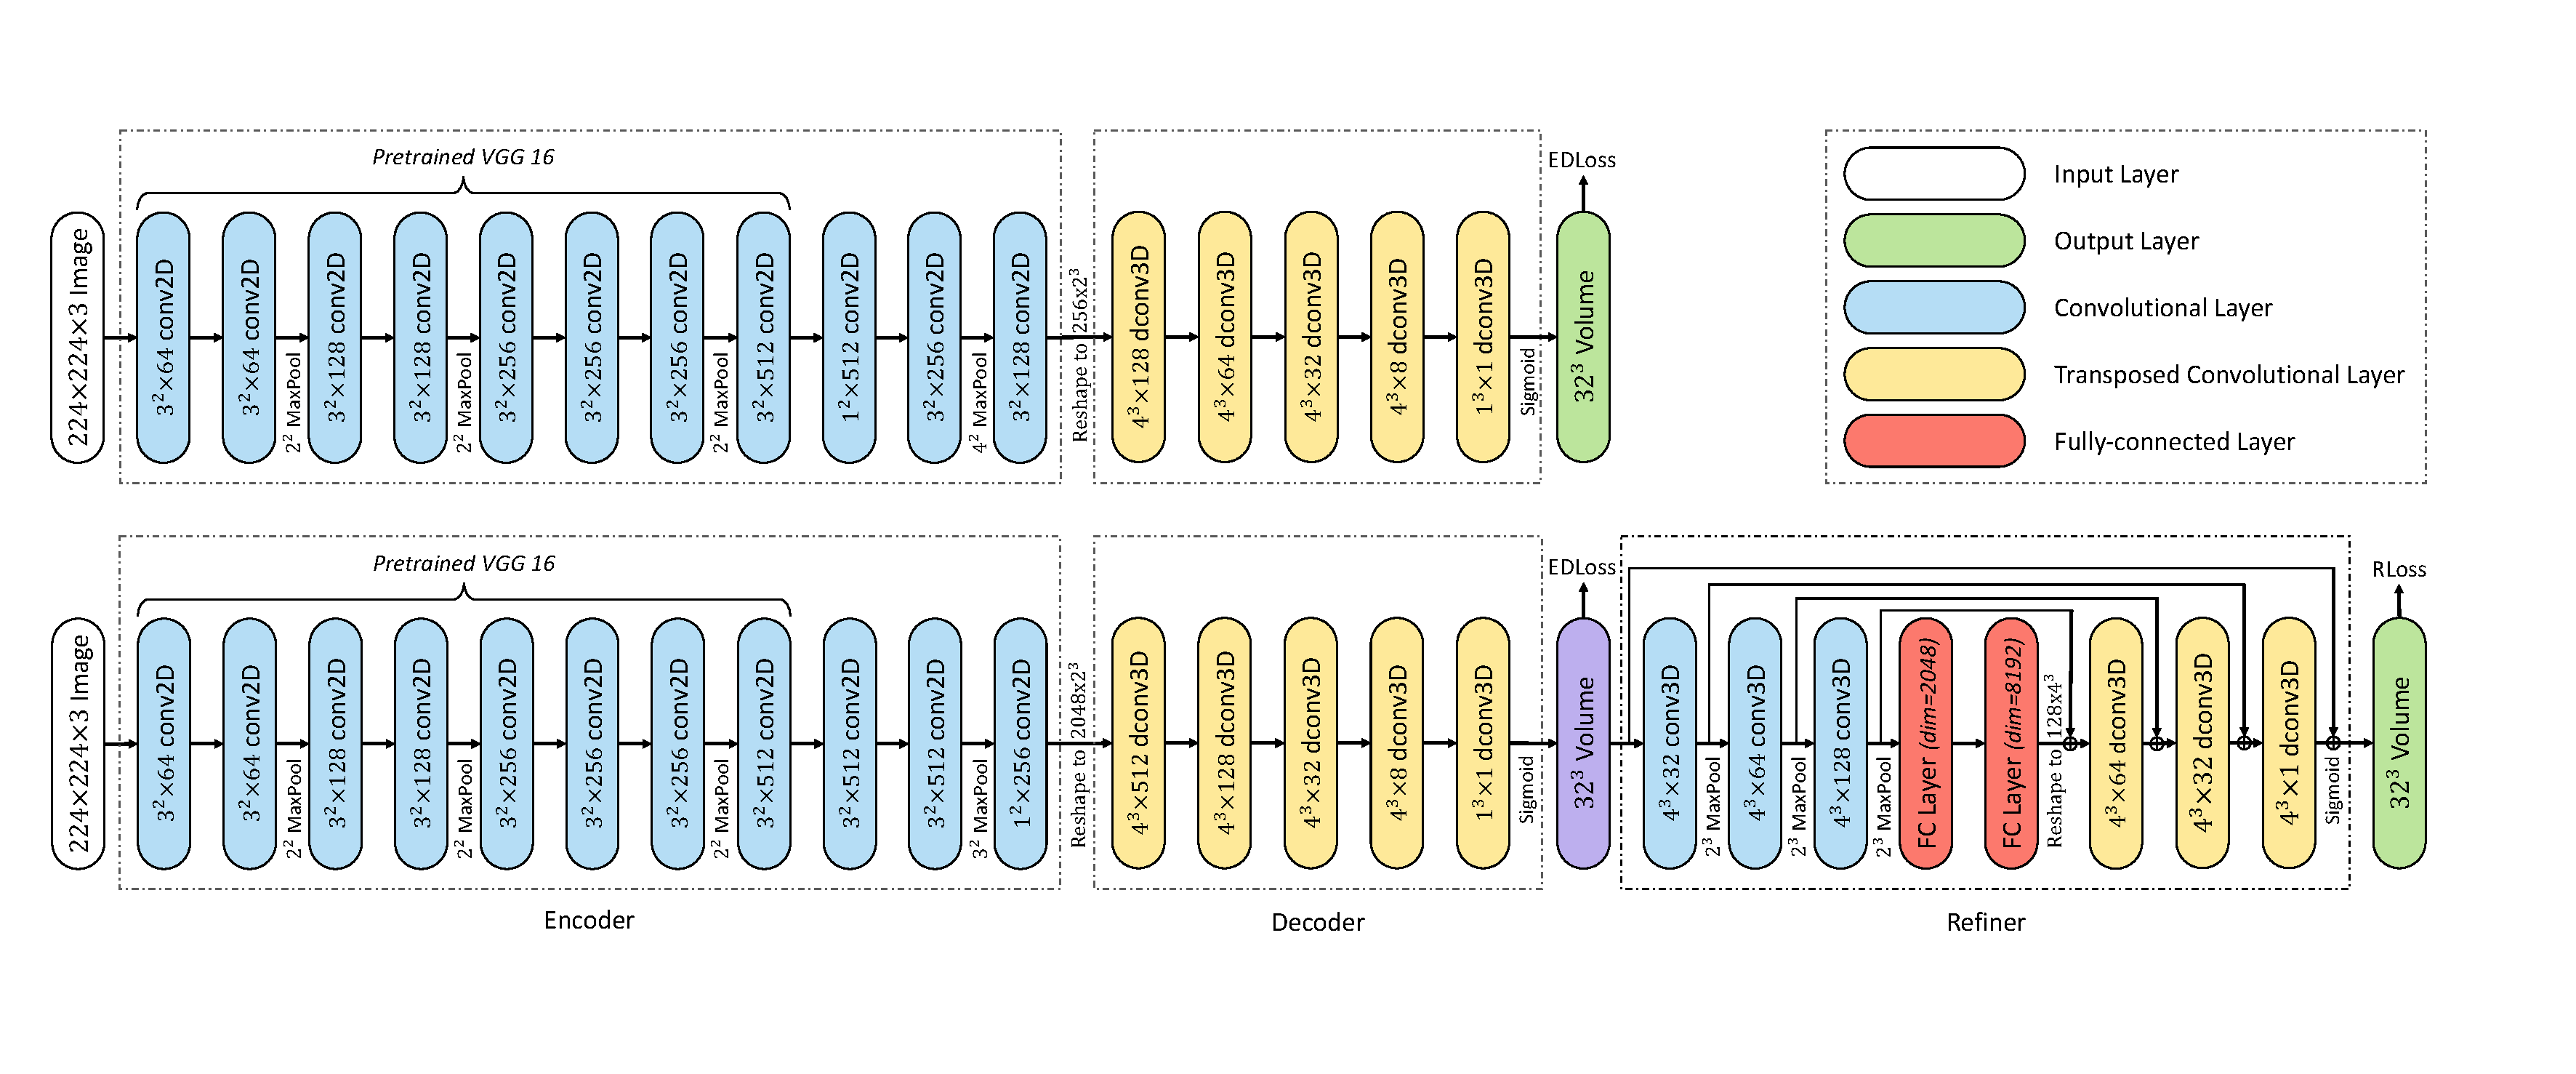
\includegraphics[angle=-90,width=0.45\linewidth]{/Users/apple/OVGU/Thesis/code/3dReconstruction/report/images/concept/pix2vox}}\quad
    \subfloat[][]{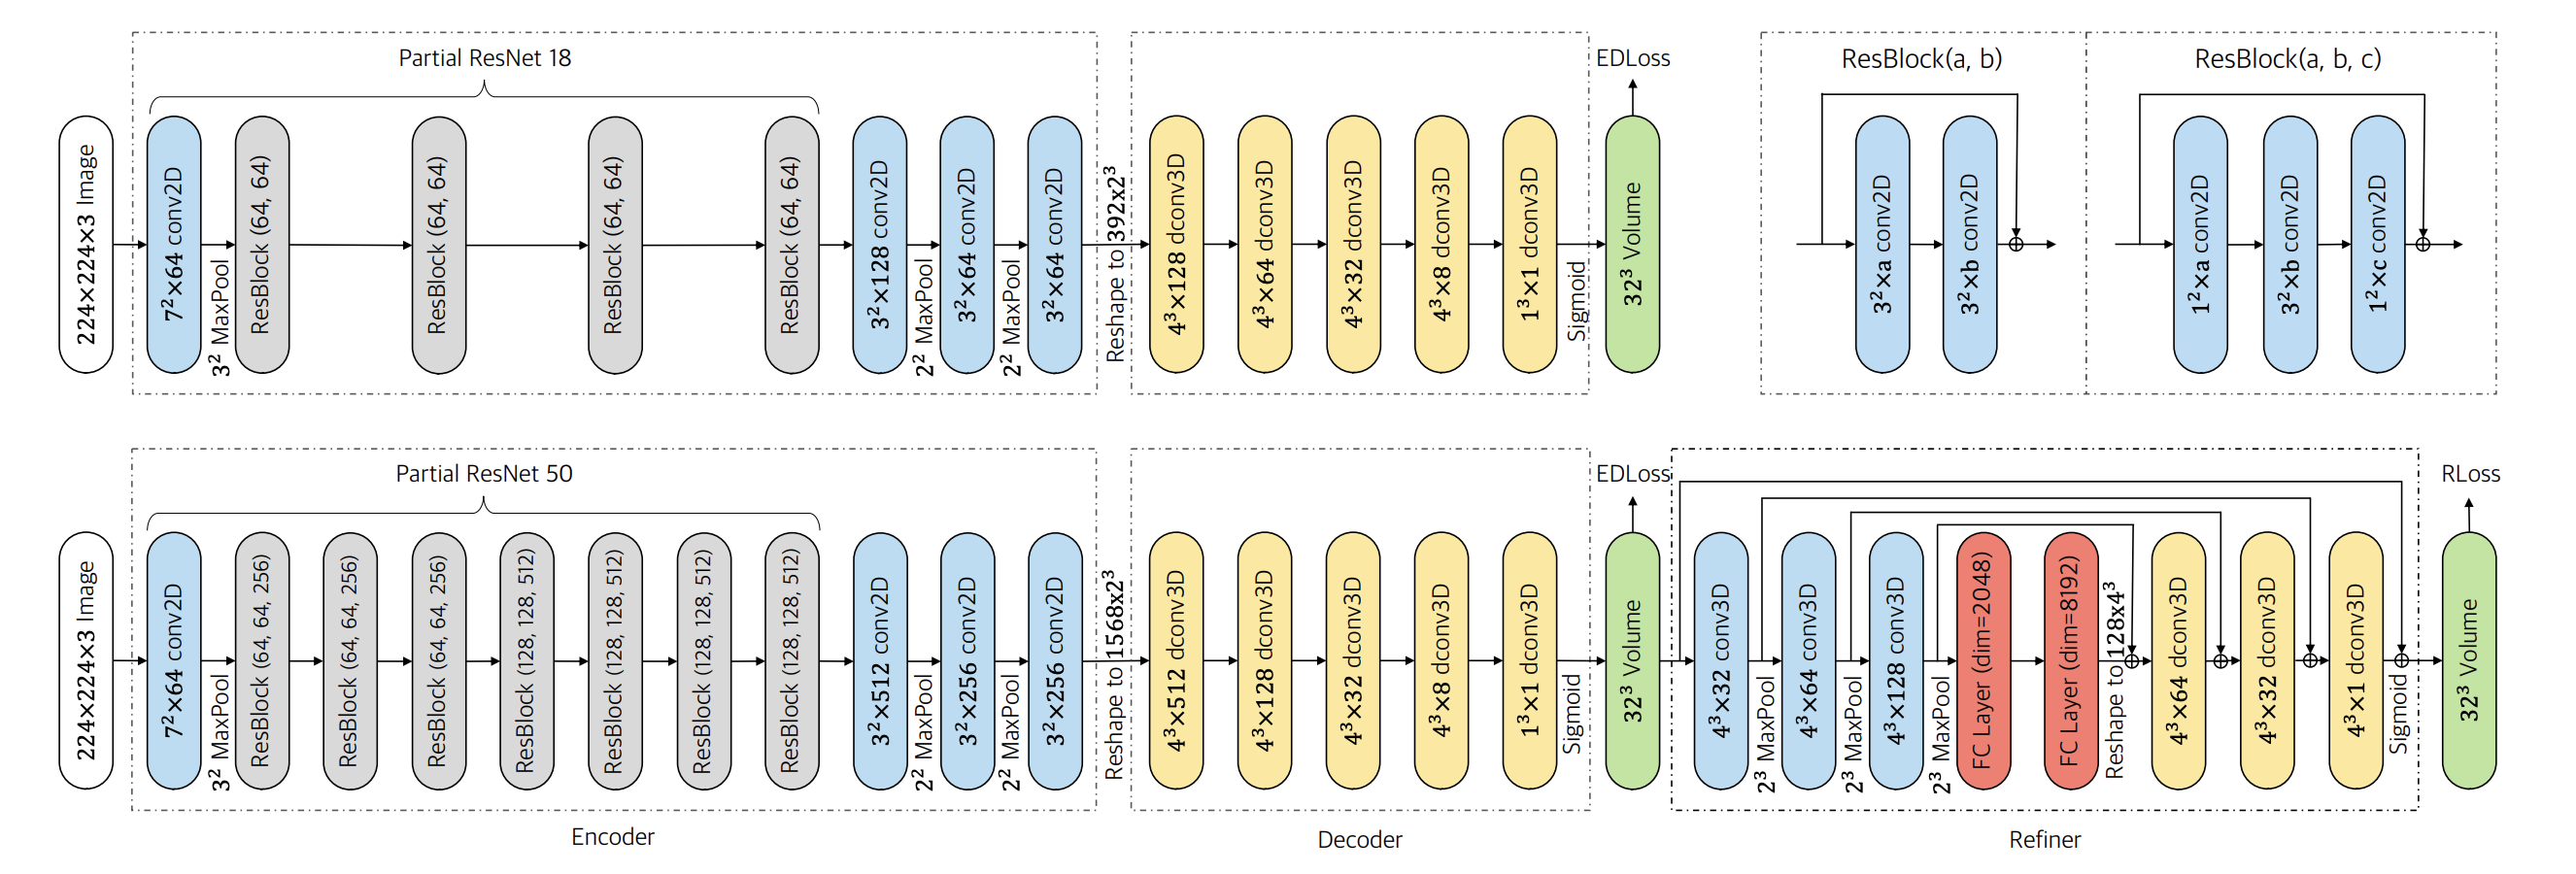
\includegraphics[angle=-90,width=0.45\linewidth]{/Users/apple/OVGU/Thesis/code/3dReconstruction/report/images/concept/pix2voxpp}}\\
    \caption{Network architectures used as a baselines (a)Pix2Vox~\cite{Xie_2019} (b)Pix2Vox++~\cite{Xie_2020}.
    The critical difference between the two architectures is the Encoder. Pix2Vox uses \gls{vgg} while Pix2Vox++ uses \gls{resnet}.}
    \label{fig:architectures}
\end{figure}

\section{Indoor datasets}\label{sec:indoor-dataset}

Now that we know what task we will be performing, lets look into existing datasets for indoor environment.
Indoor scene dataset has been on the rise with increasing interest in scene processing understanding~\cite{Dai2017,Silberman2012,Xiao2013SUN3DAD,Hua2016SceneNNAS,Armeni20163DSP,Chang2018,Handa2016UnderstandingRI,InteriorNet18,Li_2021_CVPR,zheng2020structured3d,Roberts2020HypersimAP,McCormac2017}.
The use of synthetic datasets is not something new in the world of machine learning.
As researchers realized the disadvantages of a real dataset, the focus shifted towards the synthetic dataset.
While~\cite{Dai2017, Lim2013, Sun2018} are real-world datasets,~\cite{Fu20203DFRONT3F,Handa2016UnderstandingRI,McCormac2017,Roberts2020HypersimAP} are synthetically produced.
Live scans help to gather real-world datasets.
The synthetic dataset can be manually configured by a professional or automated by a programmer using a tool.

\subsection{Pix3D: A large-scale benchmark}\label{sec:pix3d}
~\cite{Sun2018}introduces a large-scale benchmark for 2D-3D alignment.
The raw images from web search engines were collected, and labeled key points were used to align the 2D images with the corresponding 3D shapes.
The 3D models extend the IKEA dataset~\cite{Lim2013}, a collection of high-quality IKEA furniture.
The dataset also provides a binary mask and the key points for the object under observation.
To add more images to the IKEA dataset, the authors of~\cite{Sun2018} conducted a manual web search on Google, Bing, and Baidu, using the IKEA model name as keywords.
This search led to around 104,220 images which were further filtered by removing irrelevant images with the help of Amazon Mechanical Turk (AMT) workers.
After this manual experiment, the total images in Pix3D, only 14,600 images were selected for the 219 Ikea models.
Samples from Pix2D are as shown in \autoref{fig:Pix3D samples}.

\begin{figure}[!ht]
    \centering
    \subfloat[][]{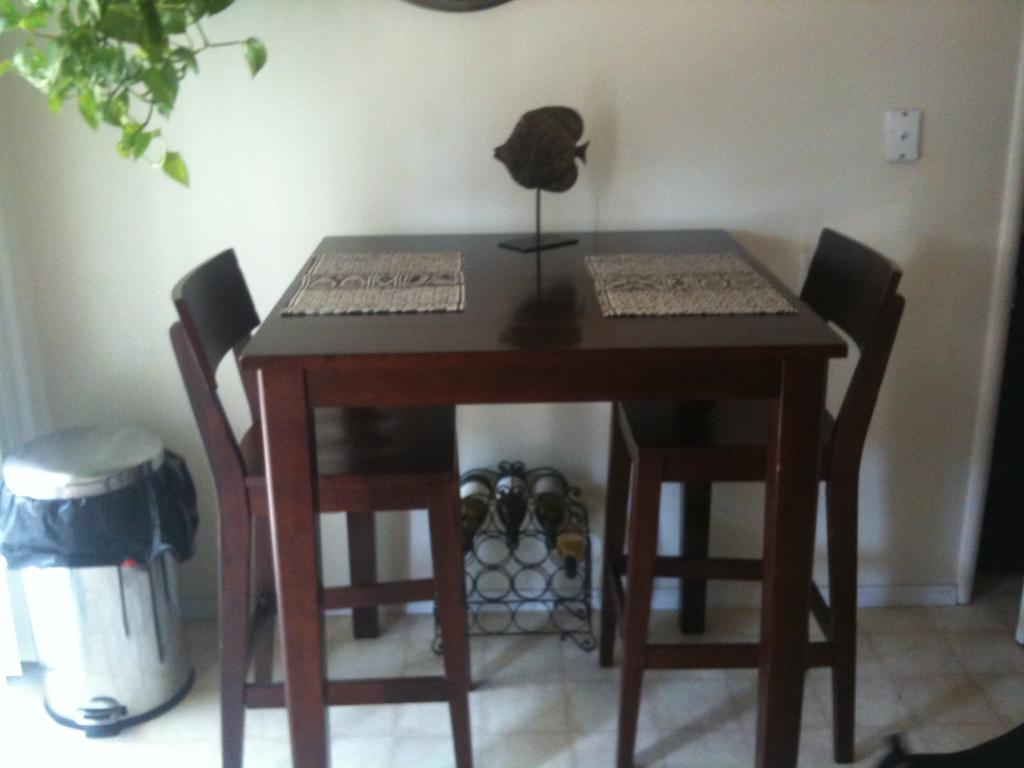
\includegraphics[width=.4\textwidth]{/Users/apple/OVGU/Thesis/code/3dReconstruction/report/images/pix3d/pix3d_5}}\quad
    \subfloat[][]{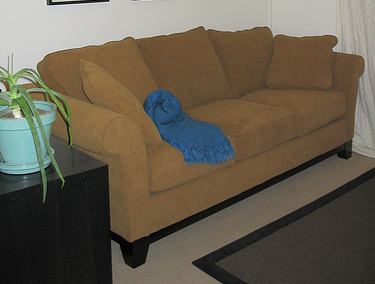
\includegraphics[width=.4\textwidth]{/Users/apple/OVGU/Thesis/code/3dReconstruction/report/images/pix3d/pix3d_2}}\\
    \subfloat[][]{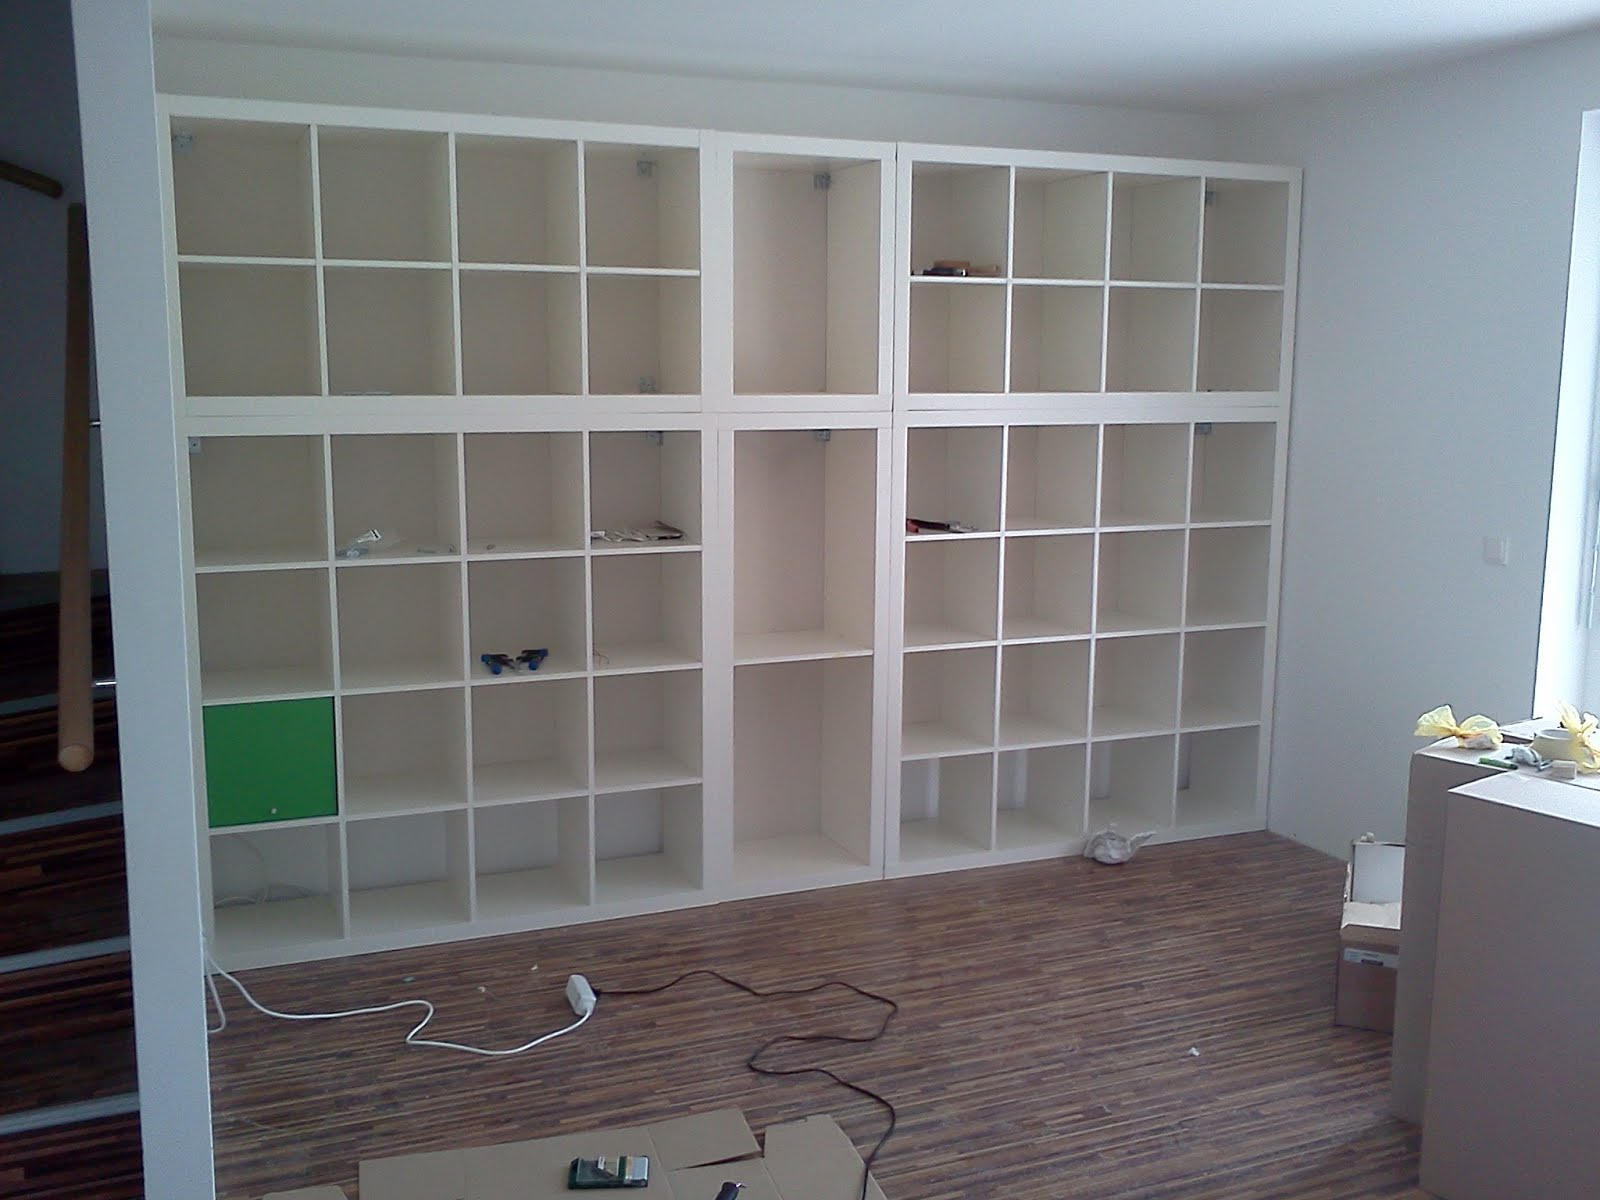
\includegraphics[width=.4\textwidth]{/Users/apple/OVGU/Thesis/code/3dReconstruction/report/images/pix3d/pix3d_6}}\quad
    \subfloat[][]{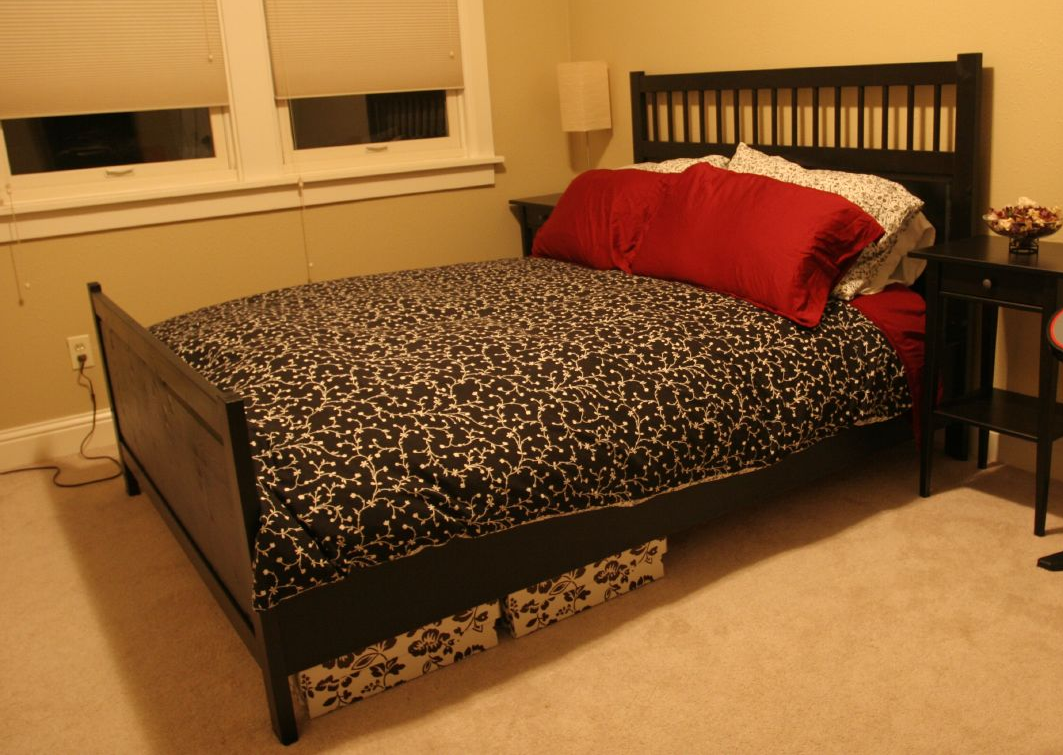
\includegraphics[width=.4\textwidth]{/Users/apple/OVGU/Thesis/code/3dReconstruction/report/images/pix3d/pix3d_4}}
    \caption{Sample RGB images from pix3D}
    \label{fig:Pix3D samples}
\end{figure}

\subsection{Indoor synthetic datasets}\label{subsec:indoor-synthetic-datasets}
Alibaba group introduced \gls{front}~\cite{Fu20203DFRONT3F} which stands for 3D Furnished Rooms with layOuts and semaNTics dataset which comprises
synthetic indoor scenes designed under the supervision of professionals.
It consists of 18,968 rooms and 13,151 textured pieces of furniture.

SceneNet~\cite{McCormac2017} is an extensive collection of photorealistic images and trajectories.
The dataset provides images and videos of indoor scenes that can be used for tasks like SLAM,
semantic and instance segmentation, object detection, and further enhanced for other vision problems like optical flow depth and pose estimation ~\cite{McCormac2017}).
They use ShapeNet~\cite{shapenet2015} models to occupy 57 indoor scenes, giving the scene unlimited configurations.
Unfortunately, there is no mapping from scene to 3D model for tasks like 3D reconstructions.

SunCG~\cite{Song2017SemanticSC} was a fundamental dataset for scene understanding.
The dataset contained over 45,000 variations of scenes with realistic room layouts created manually.
Each scene was semantically labeled and also provided with volumetric ground truth data.
We use the dataset for tasks like depth estimation, semantic scene completion, SLAM, indoor navigation, and more.
Unfortunately, due to legal issues\footnote{https://futurism.com/tech-suing-facebook-princeton-data} the dataset has been made publicly unavailable, leaving a void in the field.

Structure3D~\cite{zheng2020structured3d} is another impressive synthetic data for indoor scenes which introduced their own photorealistic renderer.
The dataset comprises 21,835 rooms in 3,500 scenes and 196k 2D images rendered with photorealism.
However, the CAD models of the 3D furniture used to populate the scenes are not made available to the public.
Hence, we cannot perform the tasks related to  3D reconstruction.
\cite{zheng2020structured3d} have also demonstrated that combining synthetic and real dataset deep learning tasks for room layout estimation improved performance on benchmark datasets.
This dataset focuses more on room layout estimation and not 3D reconstruction, but with few modifications, it may well support to 3d furniture reconstruction tasks.

Openrooms~\cite{Li_2021_CVPR} use Scannet~\cite{Dai2017} as their layout foundation, retrieve corresponding models from Shapenet~\cite{shapenet2015}
and then replace the CAD model with a retrieved model with proper alignment.
They further add the reflectance and illumination properties to compose photorealistic images.
As of August 2021, only the dataset has been made public, not the generation tool or CAD models.
The underlying concept of Openrooms is to convert existing scans into photorealistic synthetic images.
We consider them our counterparts in the output images, as the framework can produce normals, depth maps, instance segmentation, and masks the same as we do.

Hypermism~\cite{Roberts2020HypersimAP} is Apple's repository for holistic indoor scene understanding.
It is a collection of synthetic scenes created with the help of a professional artist.
Evermotion\footnote{https://evermotion.org/} was the starting point for the dataset for which assets were purchased from TurboSquid\footnote{http://www.turbosquid.com}.
The dataset includes images, 3D assets, semantic instance segmentation, and a disentangled image representation with diffused lighting and shading.
Even though the 3d triangle meshes for each asset is available online, we have to purchase them to create a custom dataset.
They also admit that the cost to generate the dataset is expensive \{approximately \$57K~\cite{Roberts2020HypersimAP}\}.

InteriorNet~\cite{InteriorNet18} claims to be a photorealistic indoor scene simulator with realistic lighting and scenes which change over time.
The image dataset includes RGB, depth, and semantic segmentation.
Along with images, they also provide synthesized realistic trajectories at a video-frame rate with various motion patterns.
The simulator also supports scenes from~\cite{McCormac2017} and~\cite{Song2017SemanticSC} along with their database.

Another simulated framework for visual research is House Of inteRactions (THOR) was introduced in \gls{ai2thor}~\cite{ai2thor}.
This dataset is again an Agent focused photorealistic dataset with the critical factor being actionable objects so that agents can interact with the objects or manipulate them.
The underlying renderer for this framework is the Unity game engine.
RoboThor~\cite{robothor} is built upon \gls{ai2thor}, consisting of real scenes and its corresponding synthetic equivalent.
It helps study agents' behavior in the real world when trained on synthetic data.
Architects manually designed the scenes by taking references from photos of the real world.

Habitat: A Platform for Embodied AI Research~\cite{Savva2019} is a photorealistic 3D simulation used for training virtual agents for tasks like navigation, question answering, instruction following..
The paper introduces Habitat-Sim, which renders scenes from Matterport3d~\cite{Chang2018}, Gibson~\cite{Xia2018}, Replica~\cite{Straub2019TheRD}, and some other datasets.
The focus of the simulator is providing the agent with sensor data and allowing additional sensors as plugins.
At the foundation level, Habitat-sim uses Magnum graphics
middleware library~\footnote{https://magnum.graphics/}, which supports cross-platform on the various hardware configuration.

In \autoref{fig:photorealistic images comparison}, we can see samples from each of the datasets claimed to be photorealistic.
The images from these datasets are used in a research survey to determine the perception of humans about photorealism.
We define``Automated dataset" as a dataset which had no or limited user or professional designer inputs.
Only the 3D furntiure models assets might have been designed by professionals, but the properties of the room like lights, textures, etc, were generated automatically.
Among the datasets under consideration,
OpenRooms, SceneNet, BlenderProc are all automated datasets, including the proposed \gls{free} dataset.
Hyperism, \gls{ai2thor}, InteriorNet, and \gls{front} were manually configured and designed by professional architects.


\begin{table}[ht]
    \centering
    \begin{tabular}{|c |c |c |c|}
        \hline
        Dataset & Year & Automated \\ [0.5ex]
        \hline\hline
        Pix3D & 2018 & NO \\
        \hline
        Openrooms & 2020 & YES \\
        \hline
        \gls{ai2thor} & 2017 & NO \\
        \hline
        BlenderProc & 2019 & YES \\
        \hline
        Hyperism & 2020 & NO \\
        \hline
        \gls{front} & 2020 & NO \\
        \hline
        InteriorNet & 2018 & NO \\
        \hline
        SceneNet & 2015 & YES \\
        \hline
        \gls{free} & 2021 & YES \\[1ex]
        \hline
    \end{tabular}
    \caption{Table represents synthetic datasets and year of release, and if they are automated(i.e. created with no or limited inputs from professional designers.)}
    \label{tab:dataset_comparison}
\end{table}

\begin{figure}
\begin{tabular}{llll}
    \gls{front} & 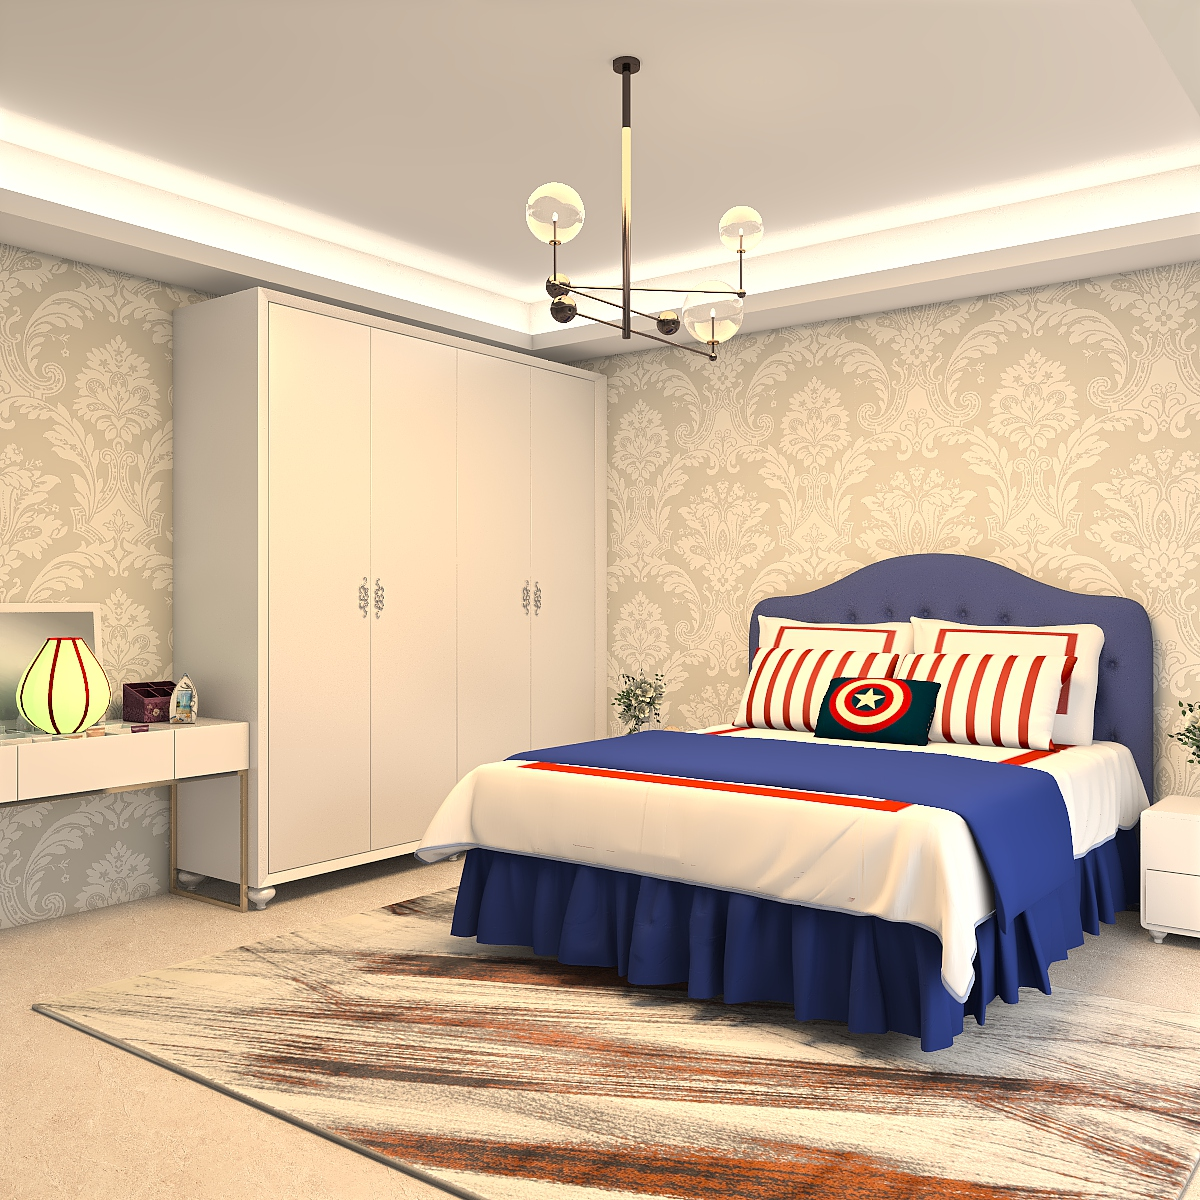
\includegraphics[width=.2\linewidth,valign=m]{/Users/apple/OVGU/Thesis/code/3dReconstruction/report/images/realistic_images_relatedwork/3dfront_1} &
    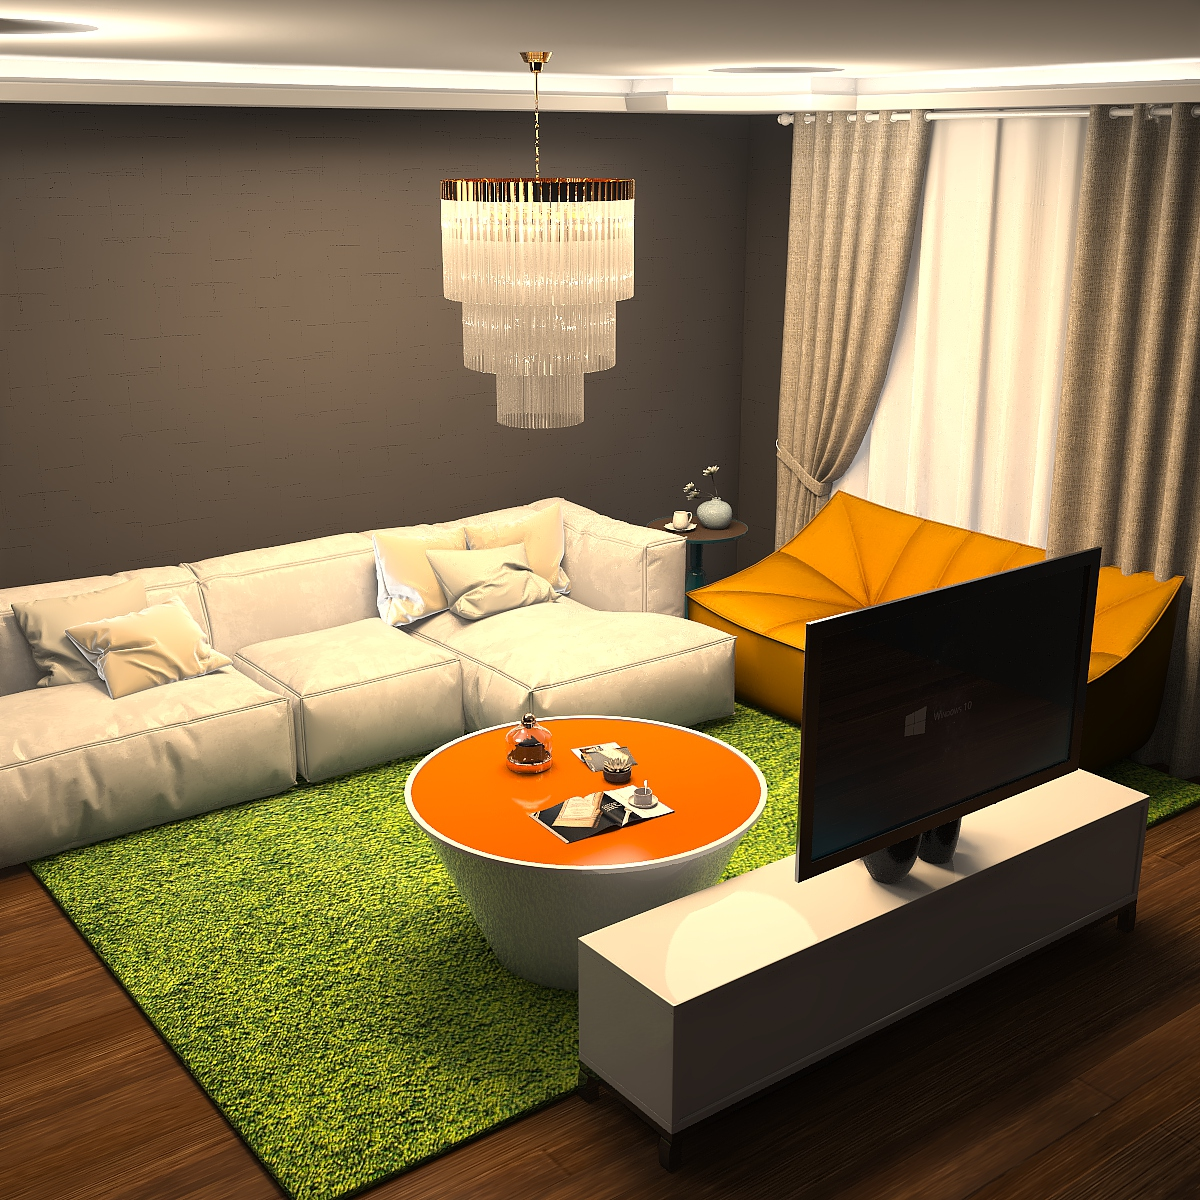
\includegraphics[width=.2\linewidth,valign=m]{/Users/apple/OVGU/Thesis/code/3dReconstruction/report/images/realistic_images_relatedwork/3dfront_2} &
    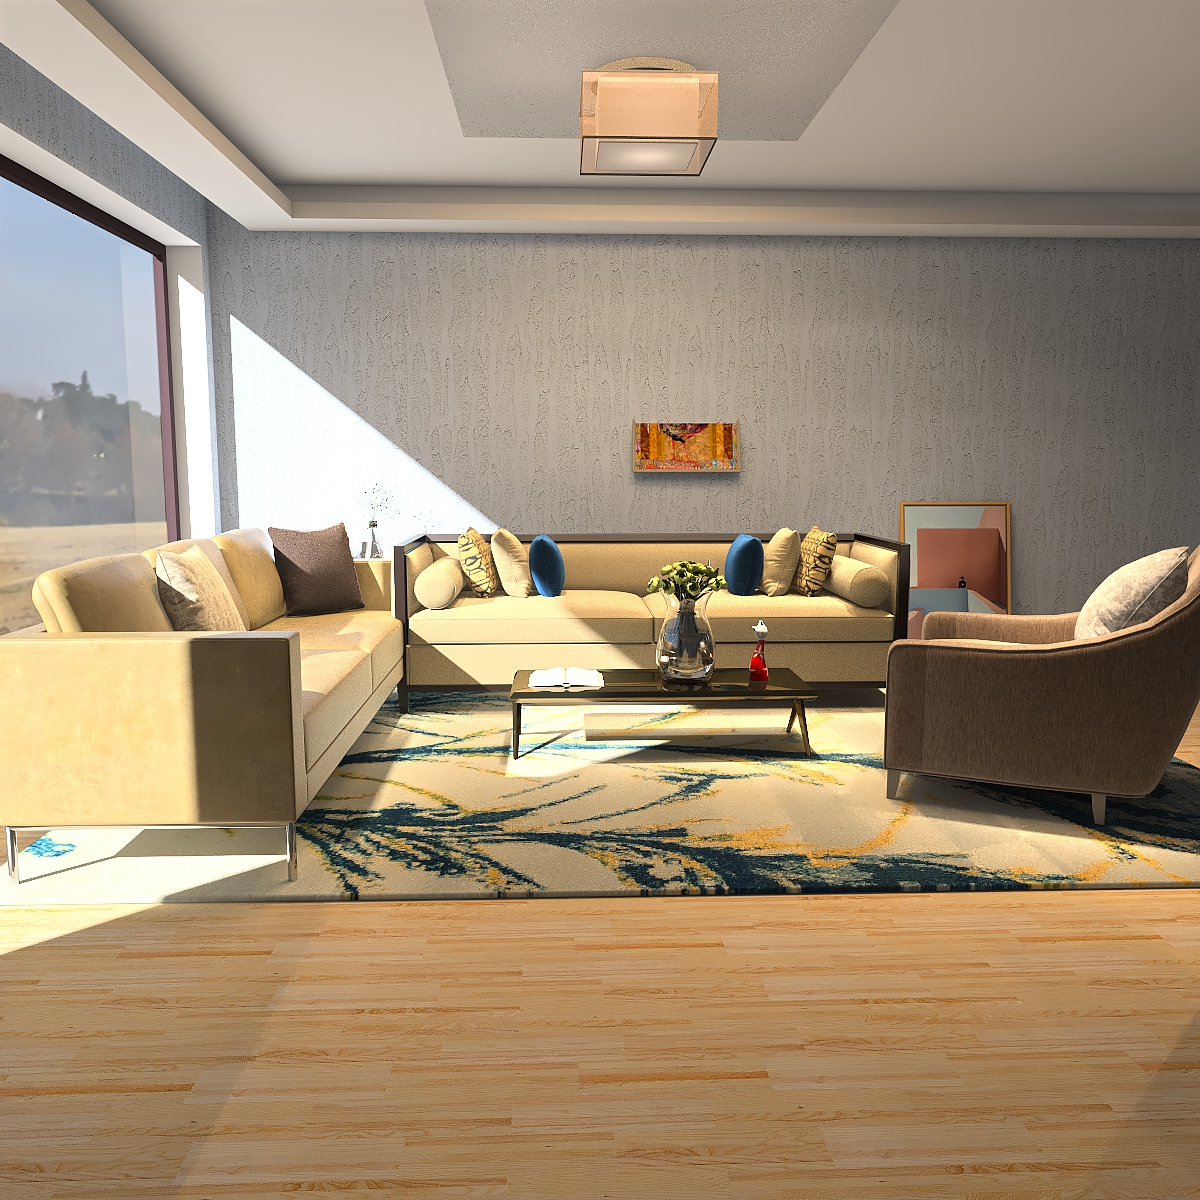
\includegraphics[width=.2\linewidth,valign=m]{/Users/apple/OVGU/Thesis/code/3dReconstruction/report/images/realistic_images_relatedwork/3dfront_3}\\

    \gls{ai2thor} & 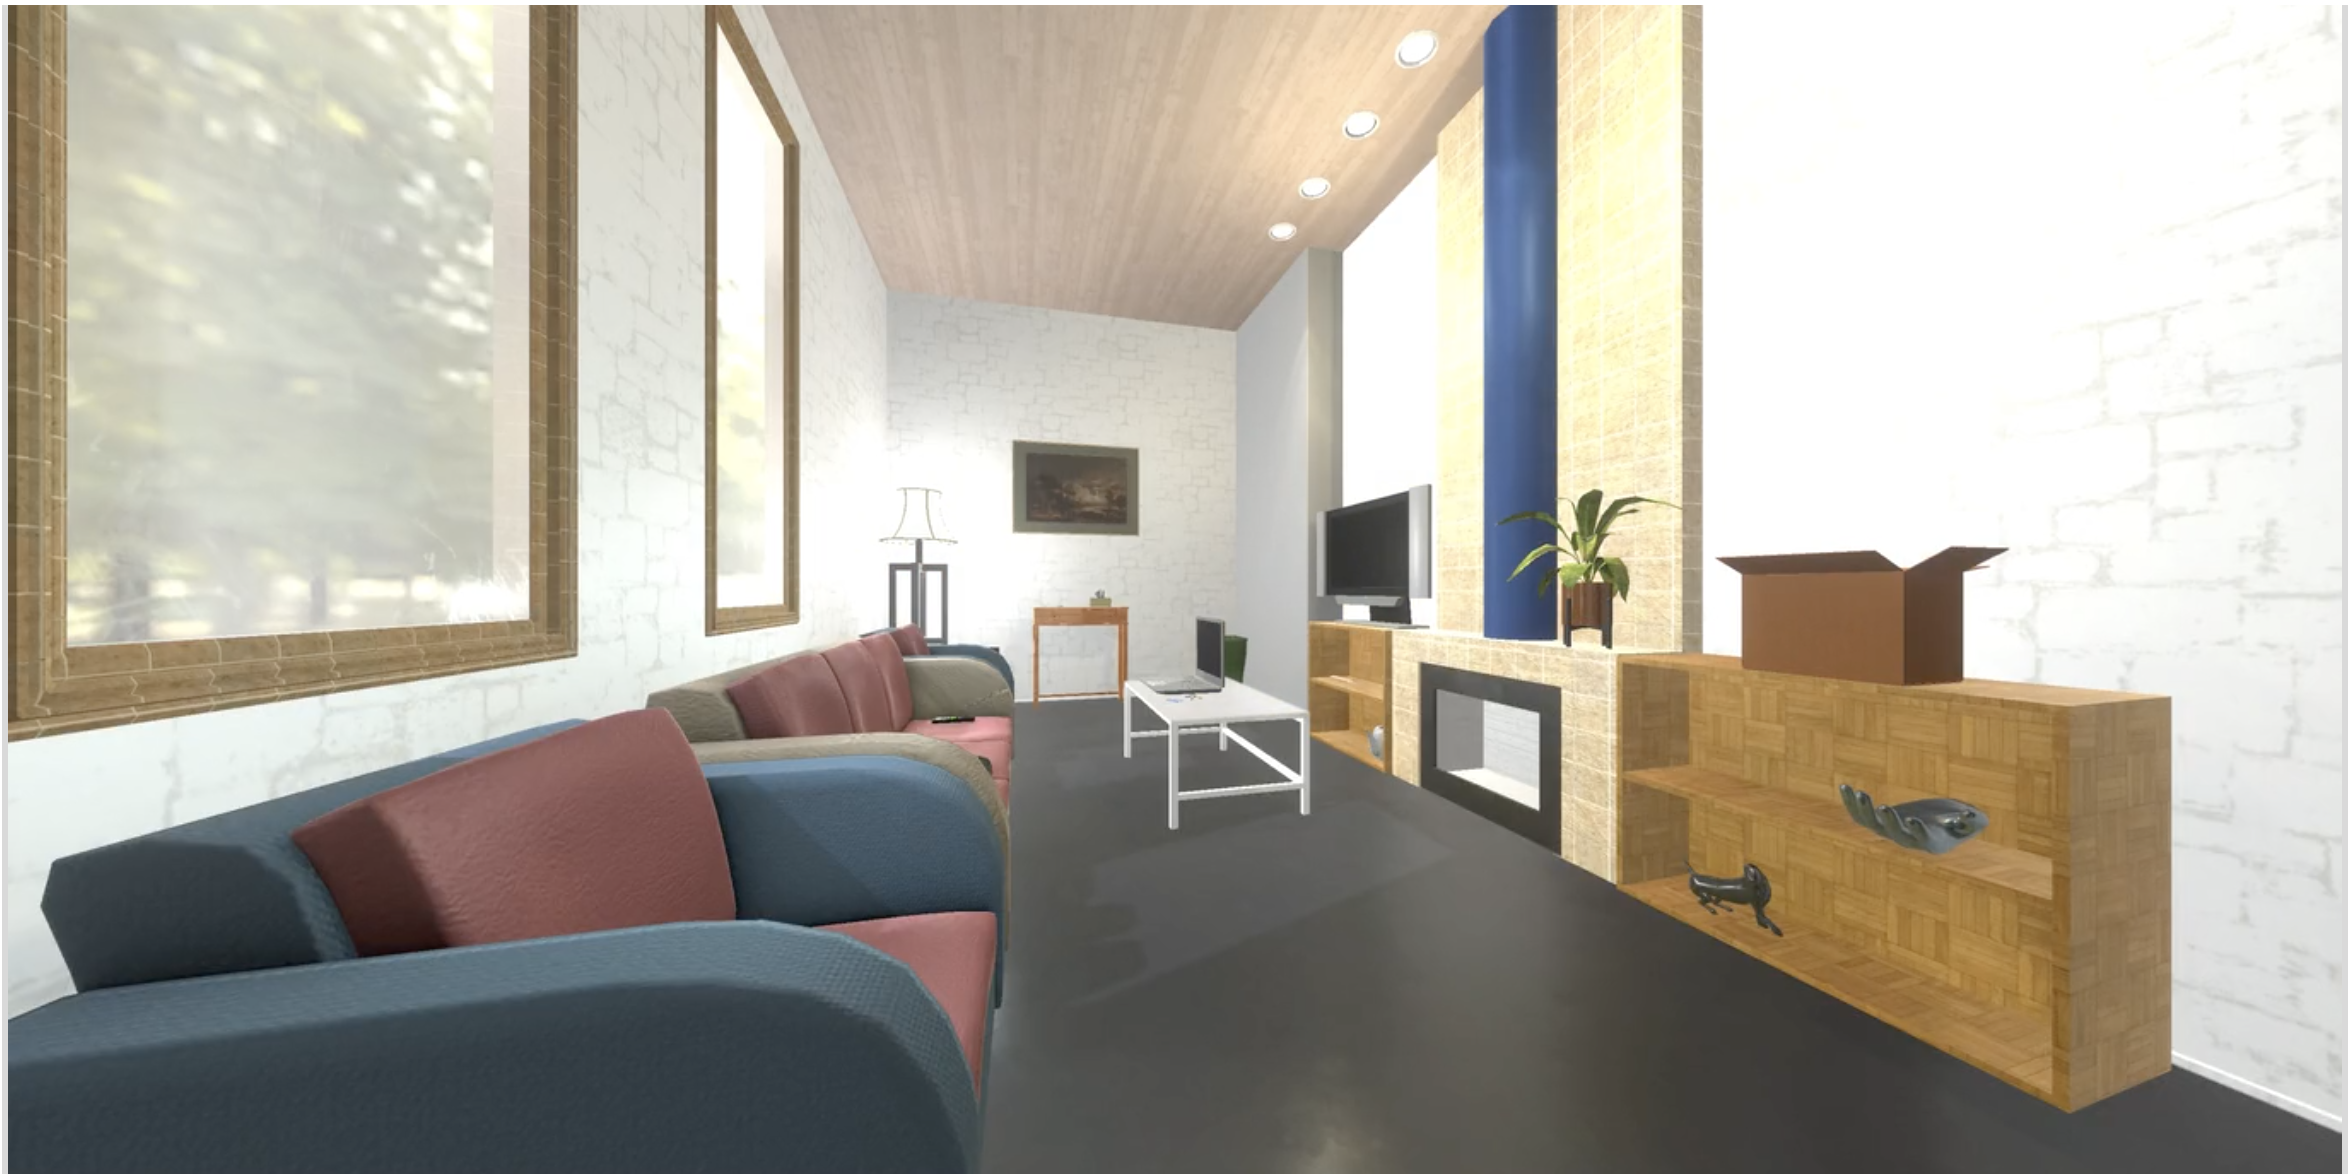
\includegraphics[width=.2\linewidth,valign=m]{/Users/apple/OVGU/Thesis/code/3dReconstruction/report/images/realistic_images_relatedwork/ai2thor_01} &
    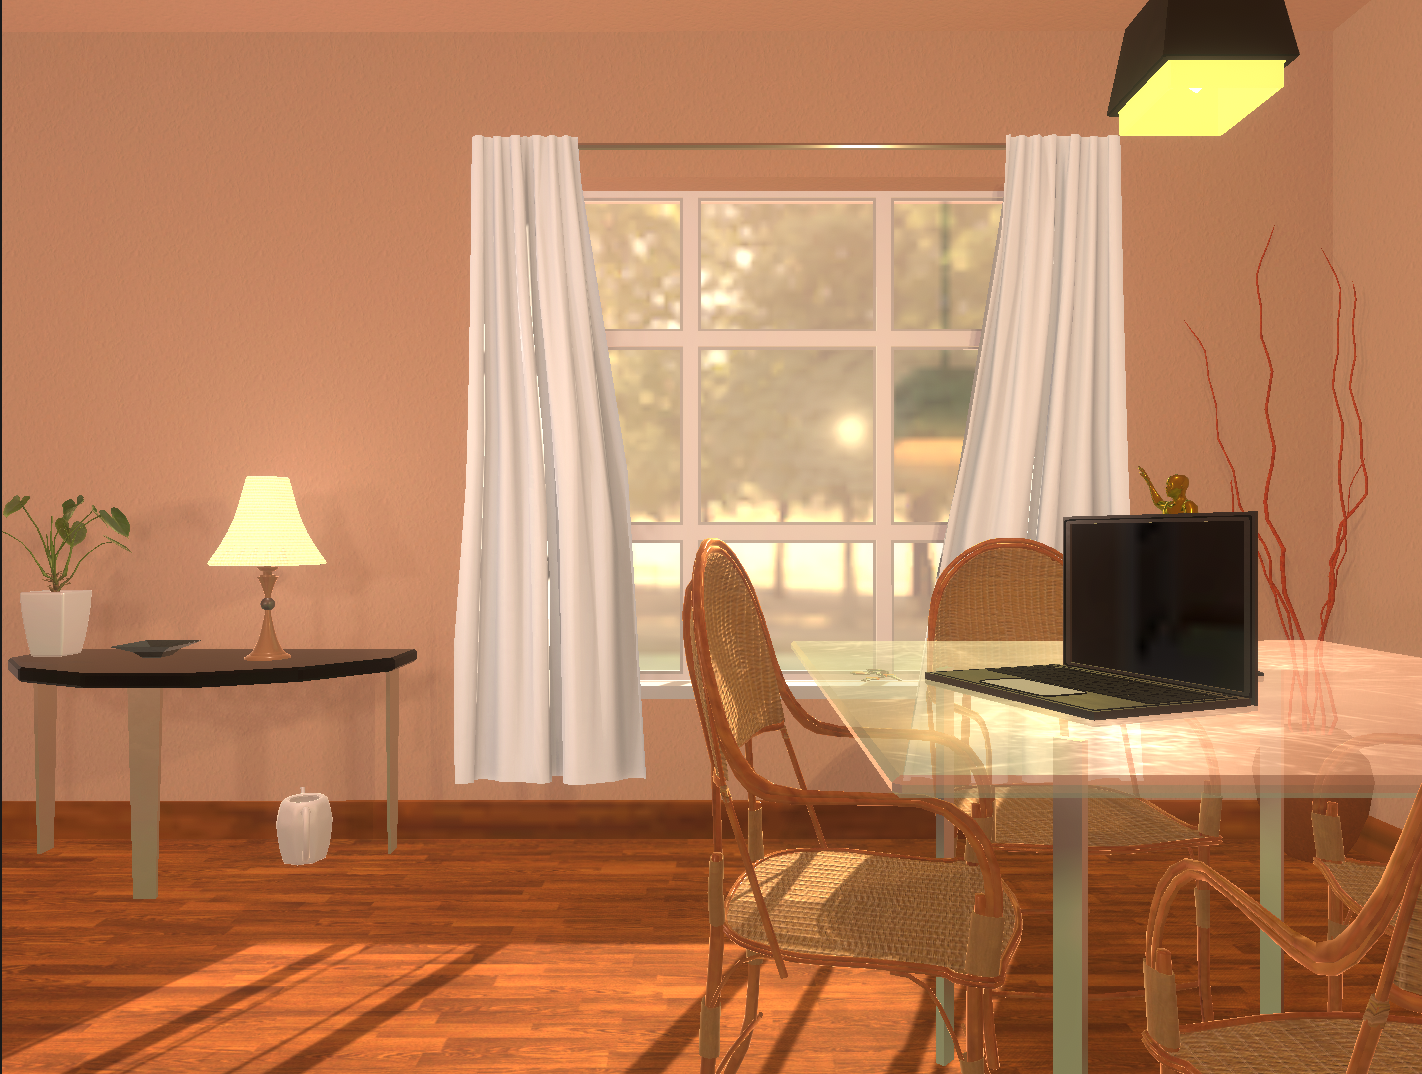
\includegraphics[width=.2\linewidth,valign=m]{/Users/apple/OVGU/Thesis/code/3dReconstruction/report/images/realistic_images_relatedwork/ai2thor_02} &
    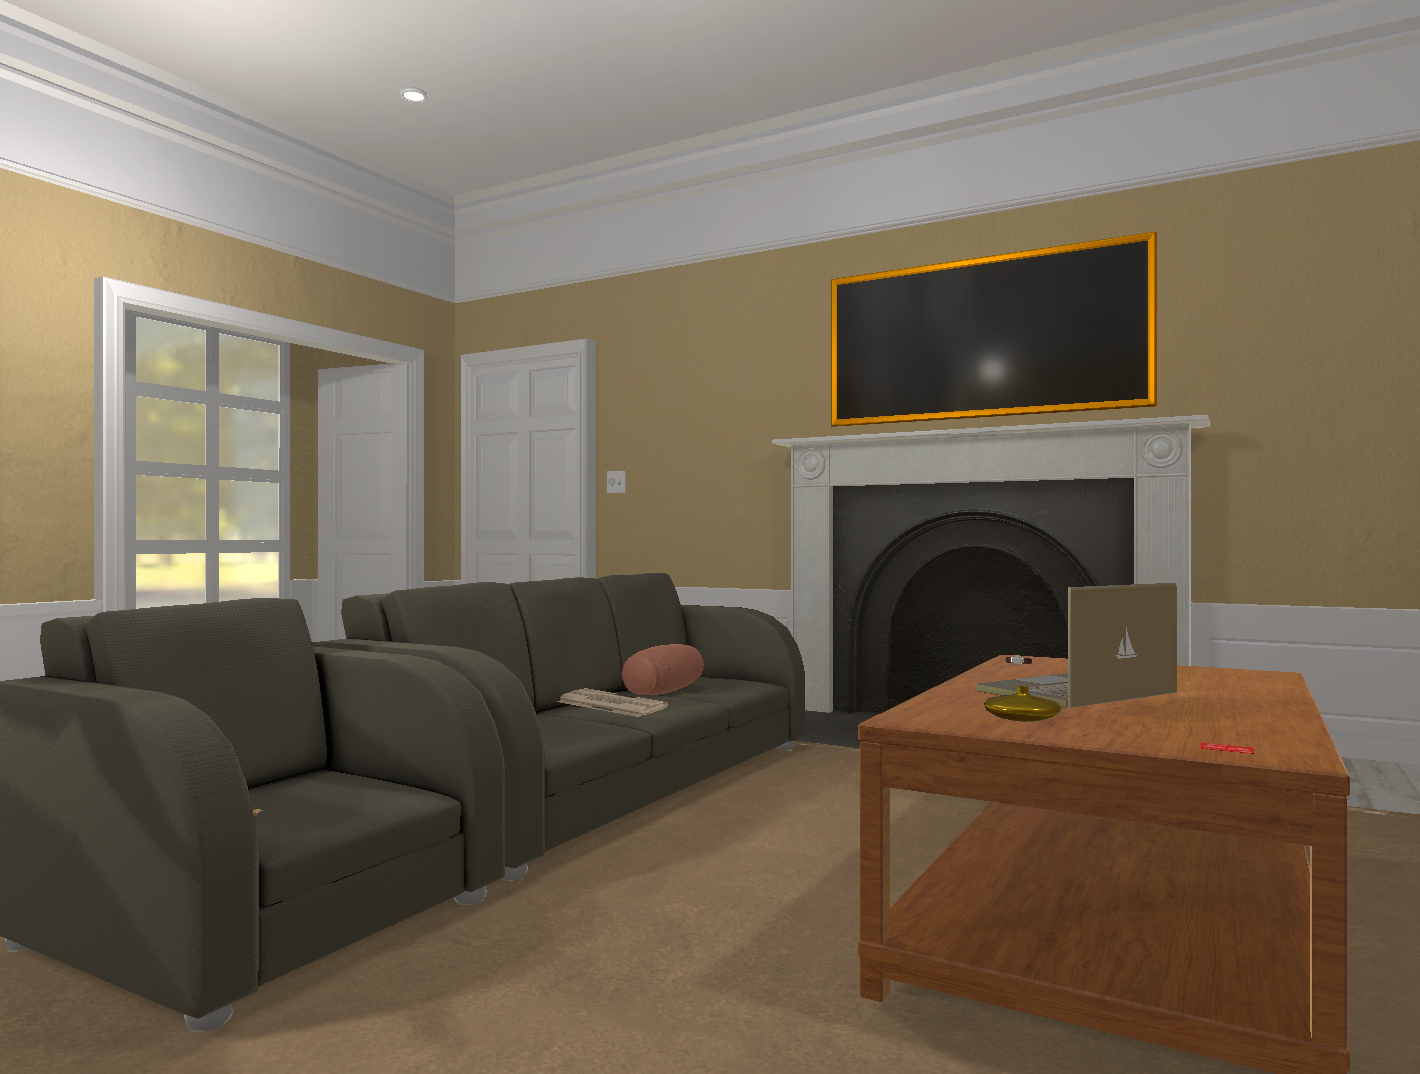
\includegraphics[width=.2\linewidth,valign=m]{/Users/apple/OVGU/Thesis/code/3dReconstruction/report/images/realistic_images_relatedwork/ai2thor_03}\\

    Hypersim & 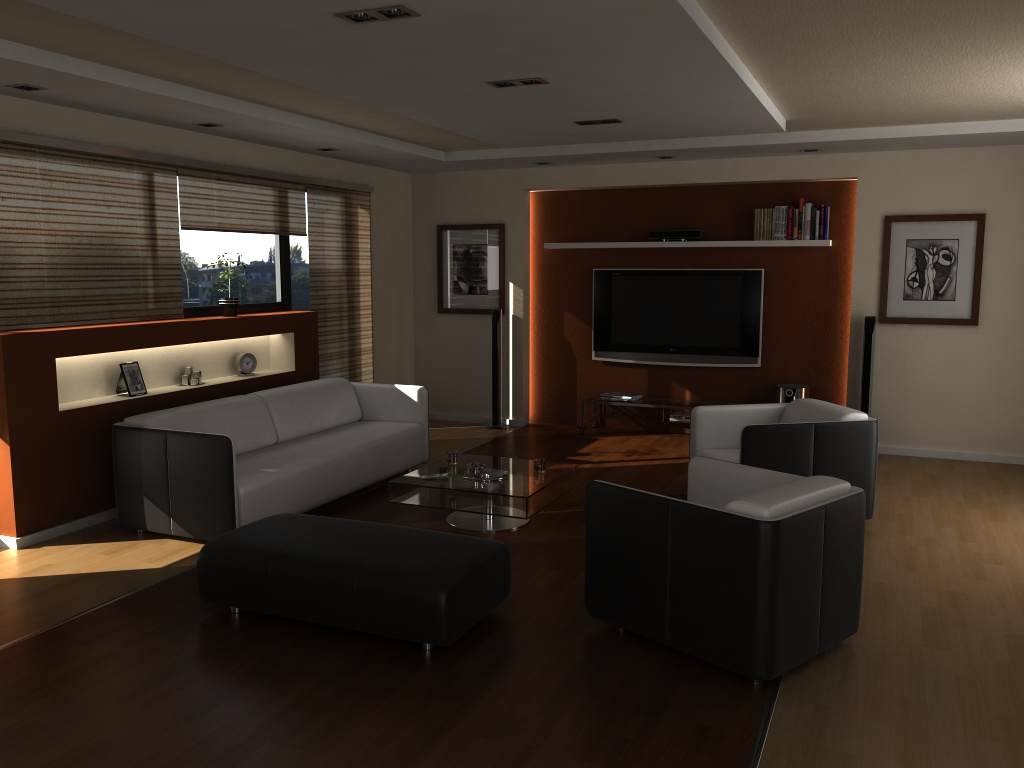
\includegraphics[width=.2\linewidth,valign=m]{/Users/apple/OVGU/Thesis/code/3dReconstruction/report/images/realistic_images_relatedwork/hypersim_01} &
    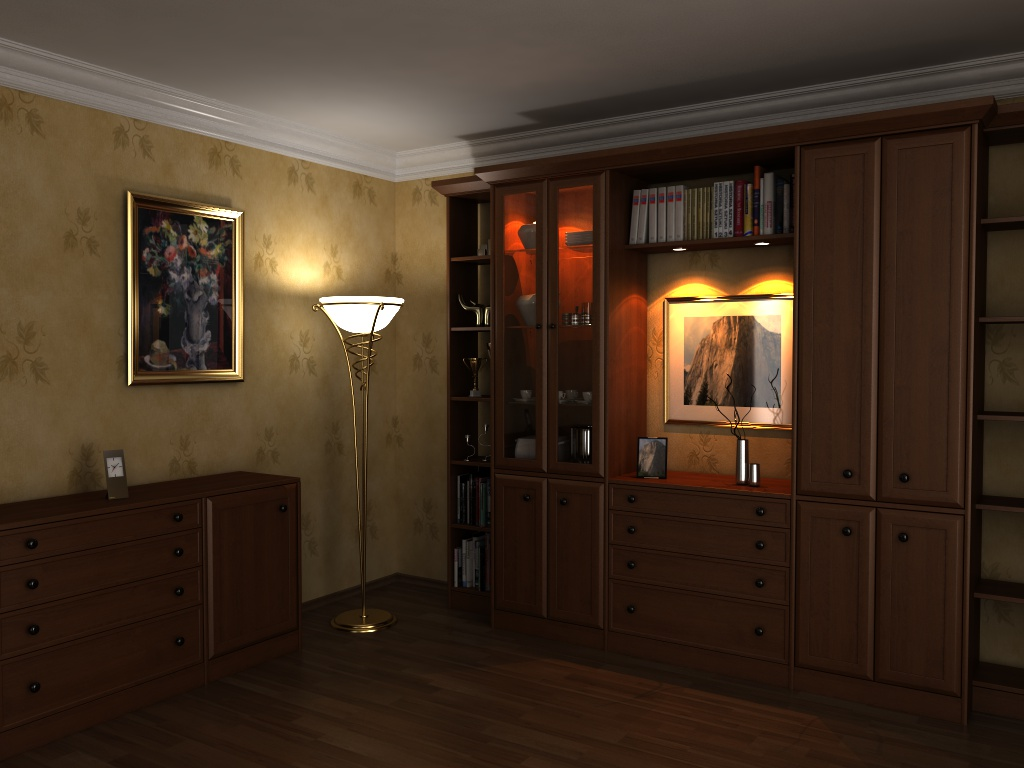
\includegraphics[width=.2\linewidth,valign=m]{/Users/apple/OVGU/Thesis/code/3dReconstruction/report/images/realistic_images_relatedwork/hypersim_02} &
    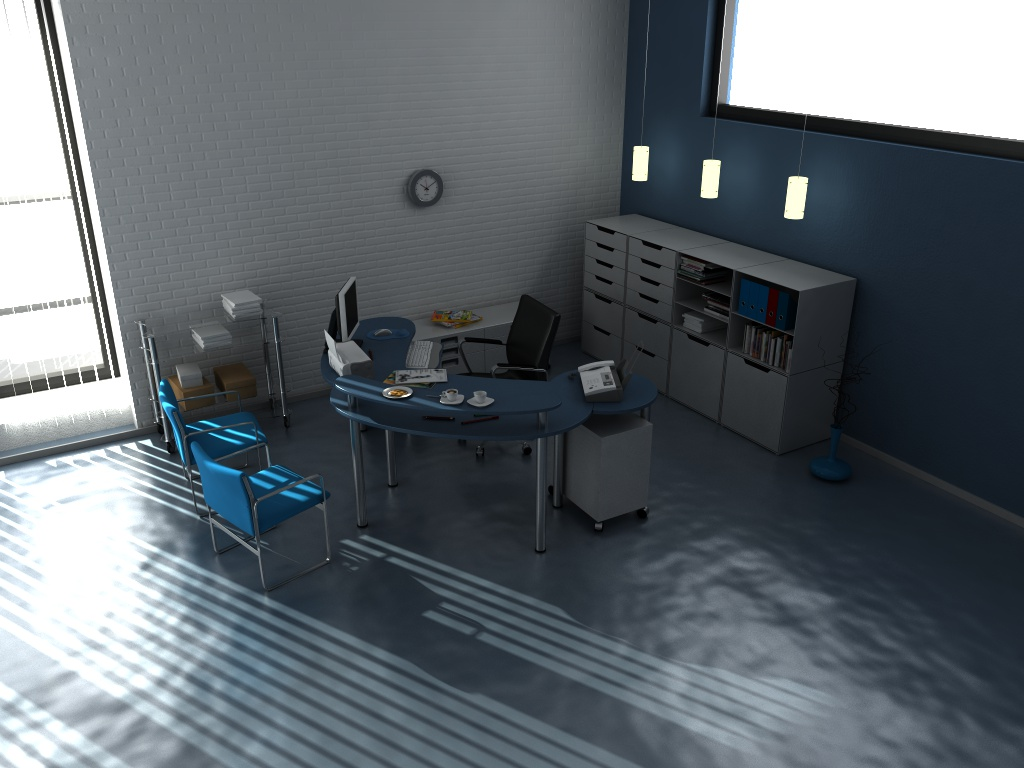
\includegraphics[width=.2\linewidth,valign=m]{/Users/apple/OVGU/Thesis/code/3dReconstruction/report/images/realistic_images_relatedwork/hypersim_03}\\

    InteriorNet & 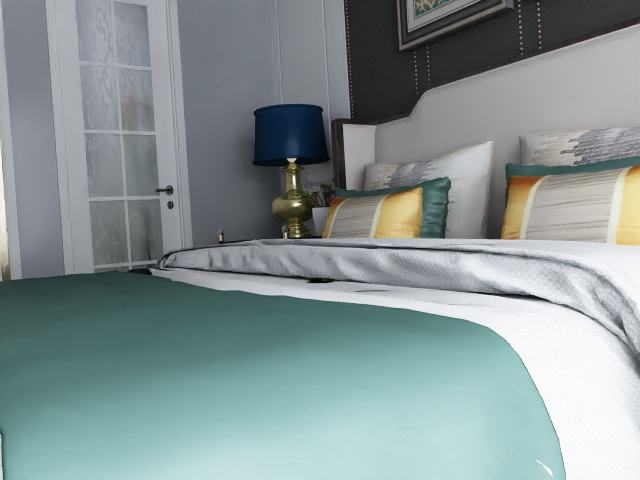
\includegraphics[width=.2\linewidth,valign=m]{/Users/apple/OVGU/Thesis/code/3dReconstruction/report/images/realistic_images_relatedwork/interiornet_01} &
    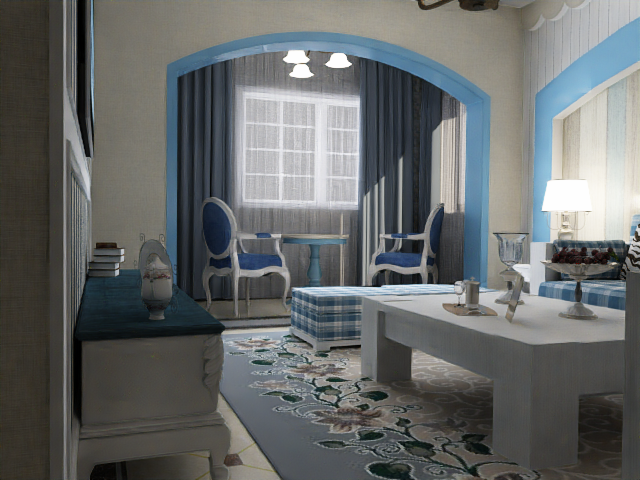
\includegraphics[width=.2\linewidth,valign=m]{/Users/apple/OVGU/Thesis/code/3dReconstruction/report/images/realistic_images_relatedwork/interiornet_02} &
    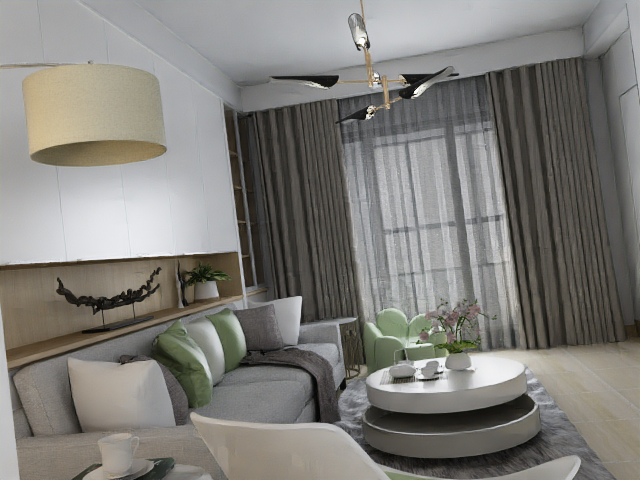
\includegraphics[width=.2\linewidth,valign=m]{/Users/apple/OVGU/Thesis/code/3dReconstruction/report/images/realistic_images_relatedwork/interiornet_03}\\

    OpenRooms & 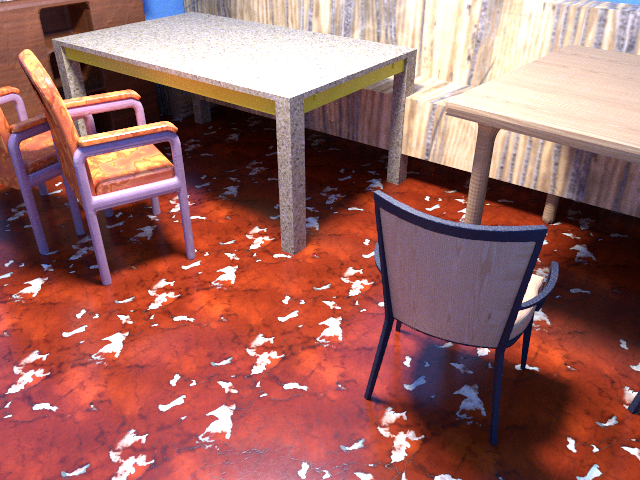
\includegraphics[width=.2\linewidth,valign=m]{/Users/apple/OVGU/Thesis/code/3dReconstruction/report/images/realistic_images_relatedwork/openrooms_01} &
    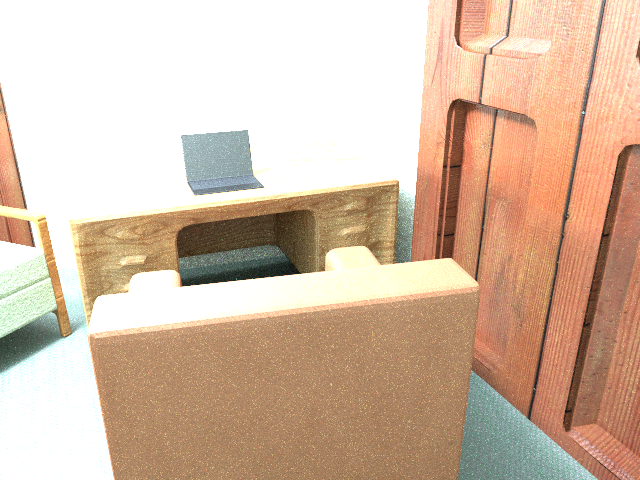
\includegraphics[width=.2\linewidth,valign=m]{/Users/apple/OVGU/Thesis/code/3dReconstruction/report/images/realistic_images_relatedwork/openrooms_02} &
    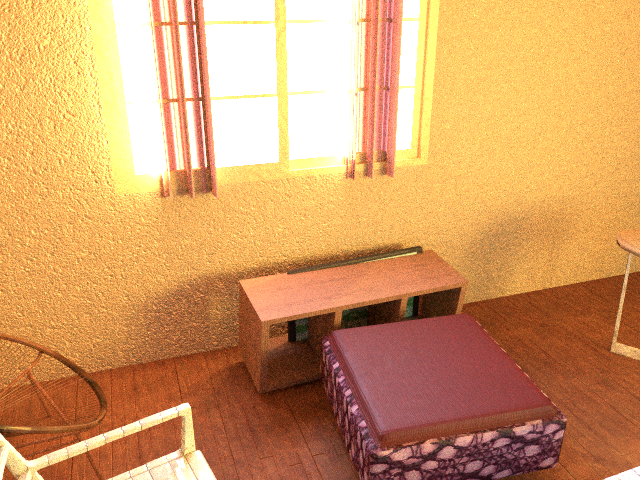
\includegraphics[width=.2\linewidth,valign=m]{/Users/apple/OVGU/Thesis/code/3dReconstruction/report/images/realistic_images_relatedwork/openrooms_03}\\

    SceneNet & 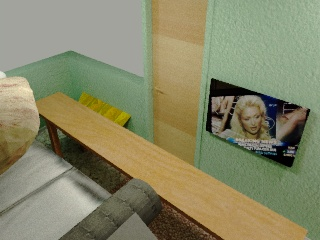
\includegraphics[width=.2\linewidth,valign=m]{/Users/apple/OVGU/Thesis/code/3dReconstruction/report/images/realistic_images_relatedwork/scenenet_1} &
    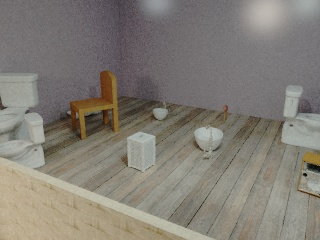
\includegraphics[width=.2\linewidth,valign=m]{/Users/apple/OVGU/Thesis/code/3dReconstruction/report/images/realistic_images_relatedwork/scenenet_2} &
    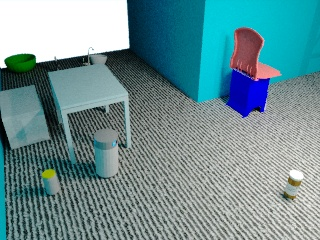
\includegraphics[width=.2\linewidth,valign=m]{/Users/apple/OVGU/Thesis/code/3dReconstruction/report/images/realistic_images_relatedwork/scenenet_3}\\

\end{tabular}
\caption{A collection of photorealistic synthetic datasets. The first column of each row indicates the dataset name followed by randomly selected images from the same dataset.}
\label{fig:photorealistic images comparison}
\end{figure}

\subsection{Tools to create synthetic datasets}\label{subsec:tools-to-create-synthetic}

``BlenderProc: Reducing the Reality Gap with Photorealistic Rendering" by ~\cite{dlr139317} is a python based pipeline to create a synthetic dataset.
As the name suggests, the underlying framework is Blender~\cite{blender}, which is a 3D modeling and rendering package.
Like most synthetic data generation tools, it provides RGB, depth maps, normals, and semantic segmentation.
\autoref{fig:Blenderproc samples} is a collection of sample images generated using BlenderPoc.
We searched for synthetic data generation tools, Blenderproc supports a maximum number of existing datasets.
Ikea~\cite{Lim2013}, Pix3d~\cite{Sun2018}, Shapenet~\cite{shapenet2015}, \gls{front}~\cite{Fu20203DFRONT3F}, Replica~\cite{Straub2019TheRD}, SunCG~\cite{Xiao2013SUN3DAD} are some of the popular datasets it supports.
It also has some combinations of these datasets like ShapeNet with SunCG or SceneNet.
Even though it supports the rendering of the Pix3D dataset, the model is rendered without any background.
One extreme advantage of this toolkit is that it is open source and a more comprehensive open community to contribute.

\begin{figure}
    \begin{tabular}{llll}
        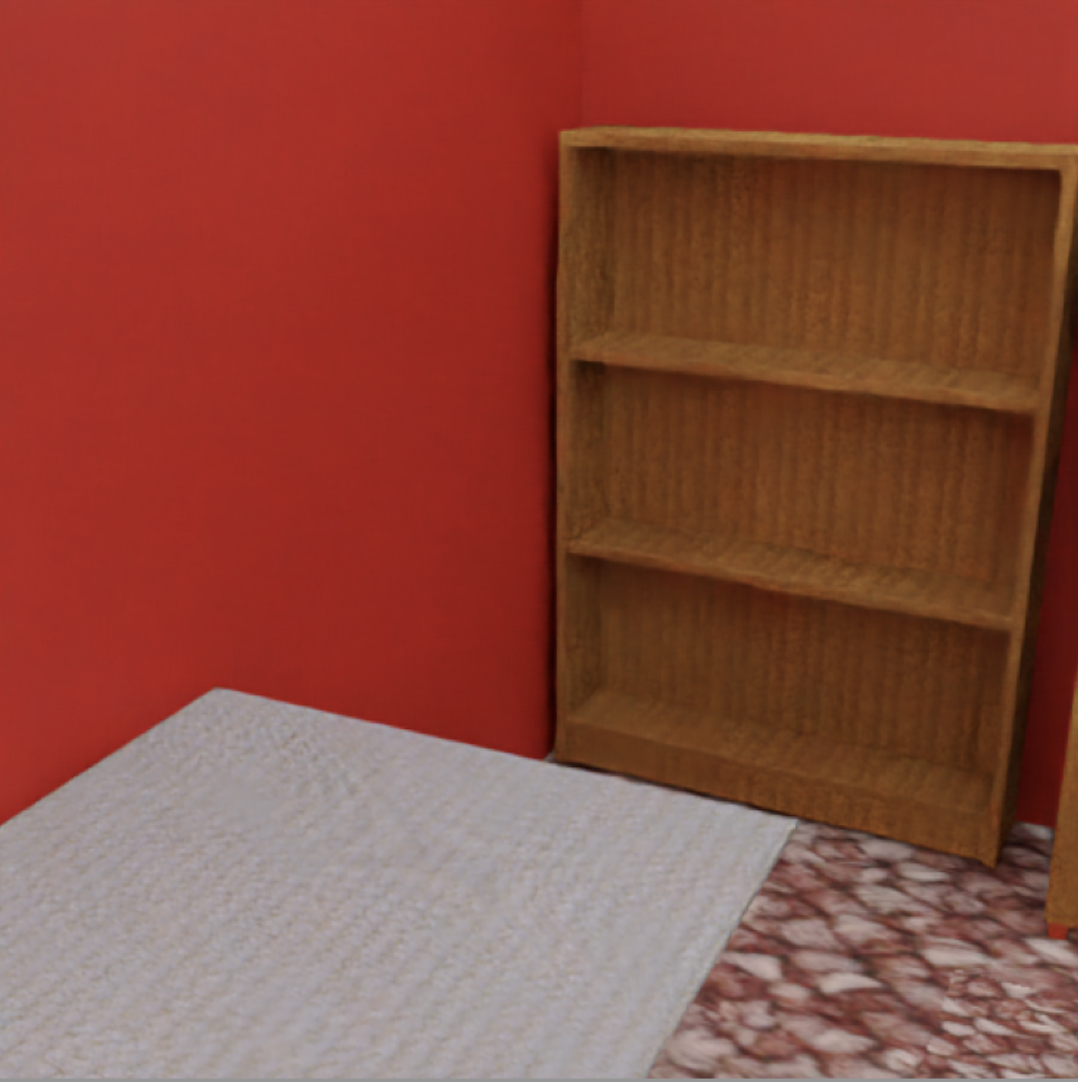
\includegraphics[width=.2\linewidth,valign=m]{/Users/apple/OVGU/Thesis/code/3dReconstruction/report/images/realistic_images_relatedwork/blenderproc_1} &
        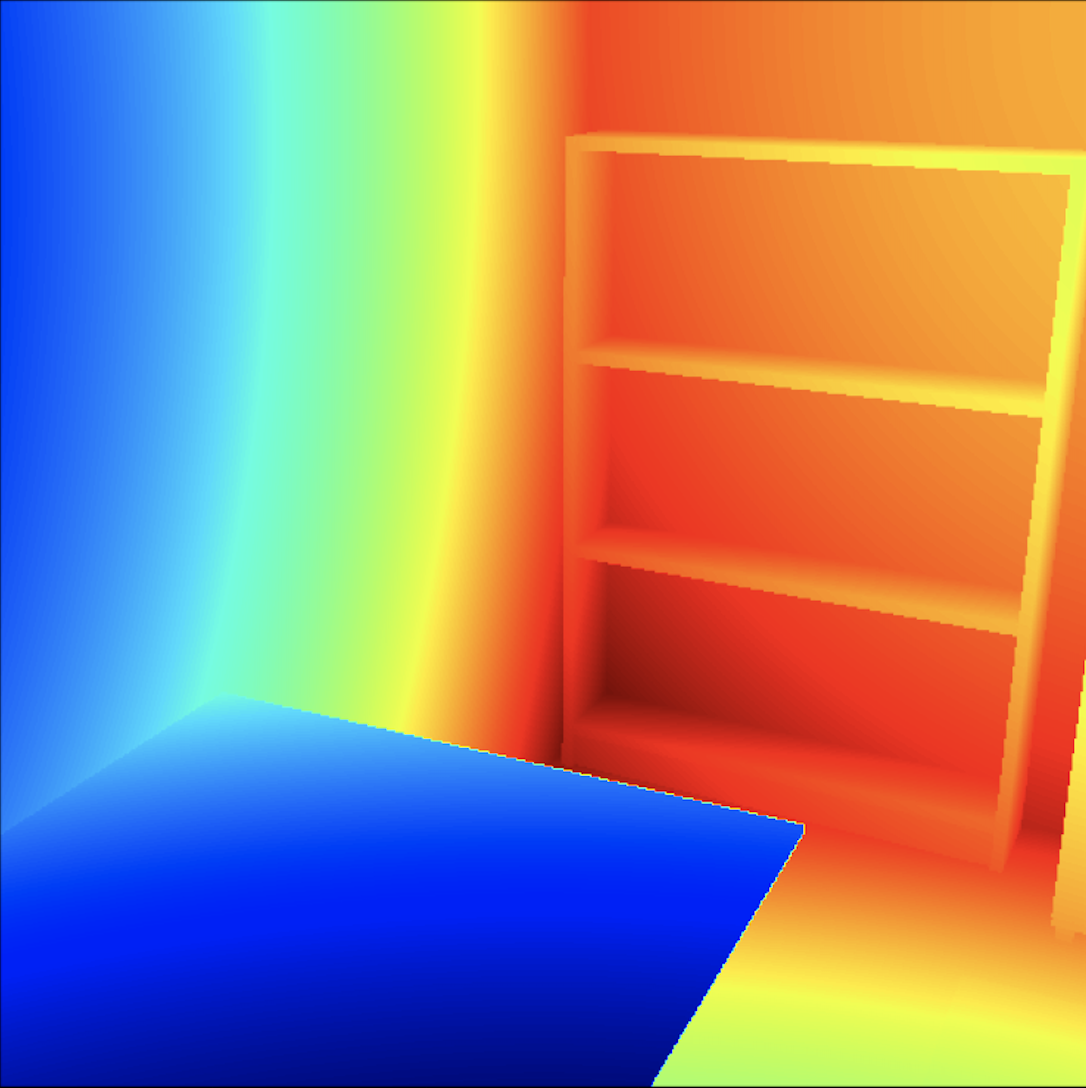
\includegraphics[width=.2\linewidth,valign=m]{/Users/apple/OVGU/Thesis/code/3dReconstruction/report/images/realistic_images_relatedwork/blenderproc_depth_1} &
        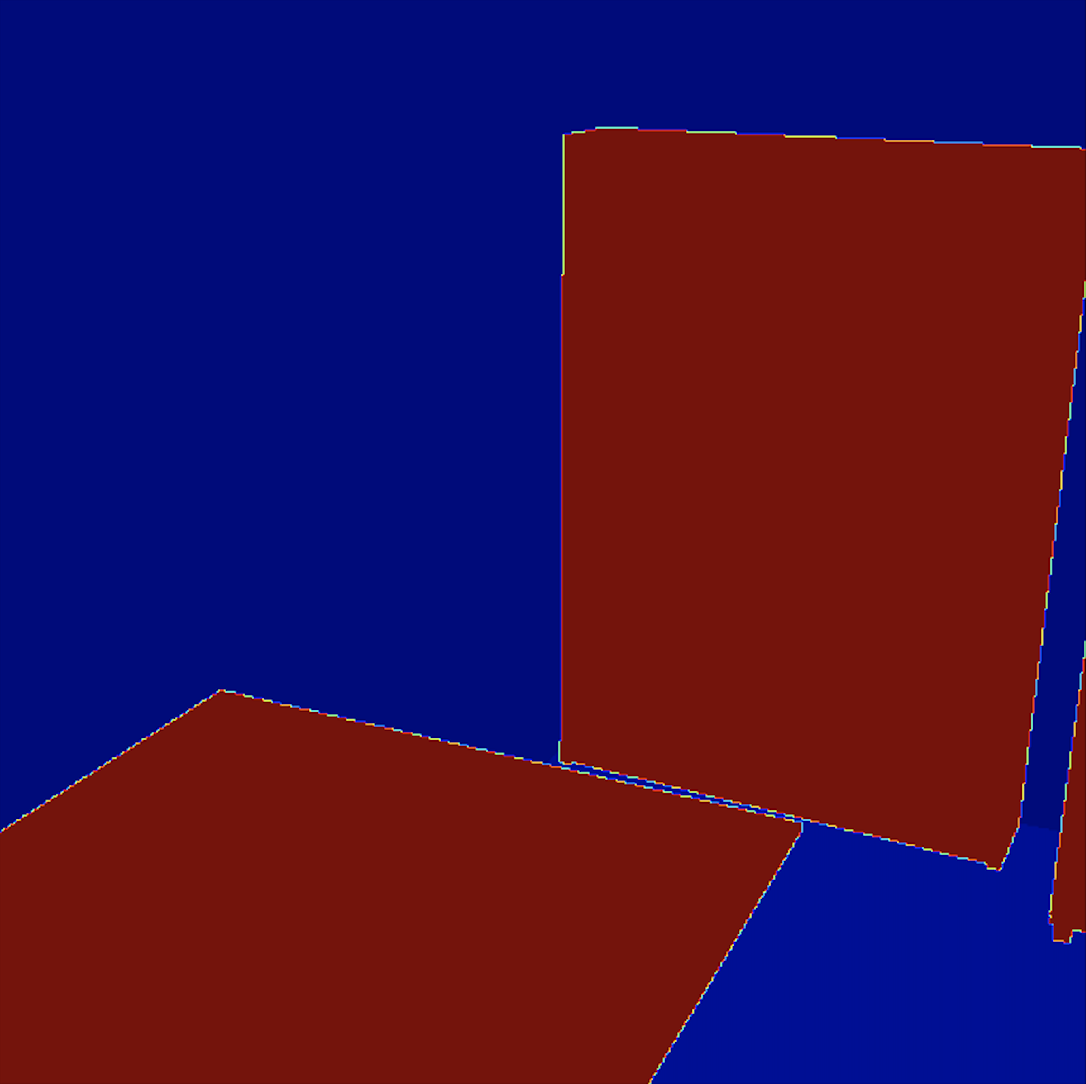
\includegraphics[width=.2\linewidth,valign=m]{/Users/apple/OVGU/Thesis/code/3dReconstruction/report/images/realistic_images_relatedwork/blenderproc_instance_1} &
        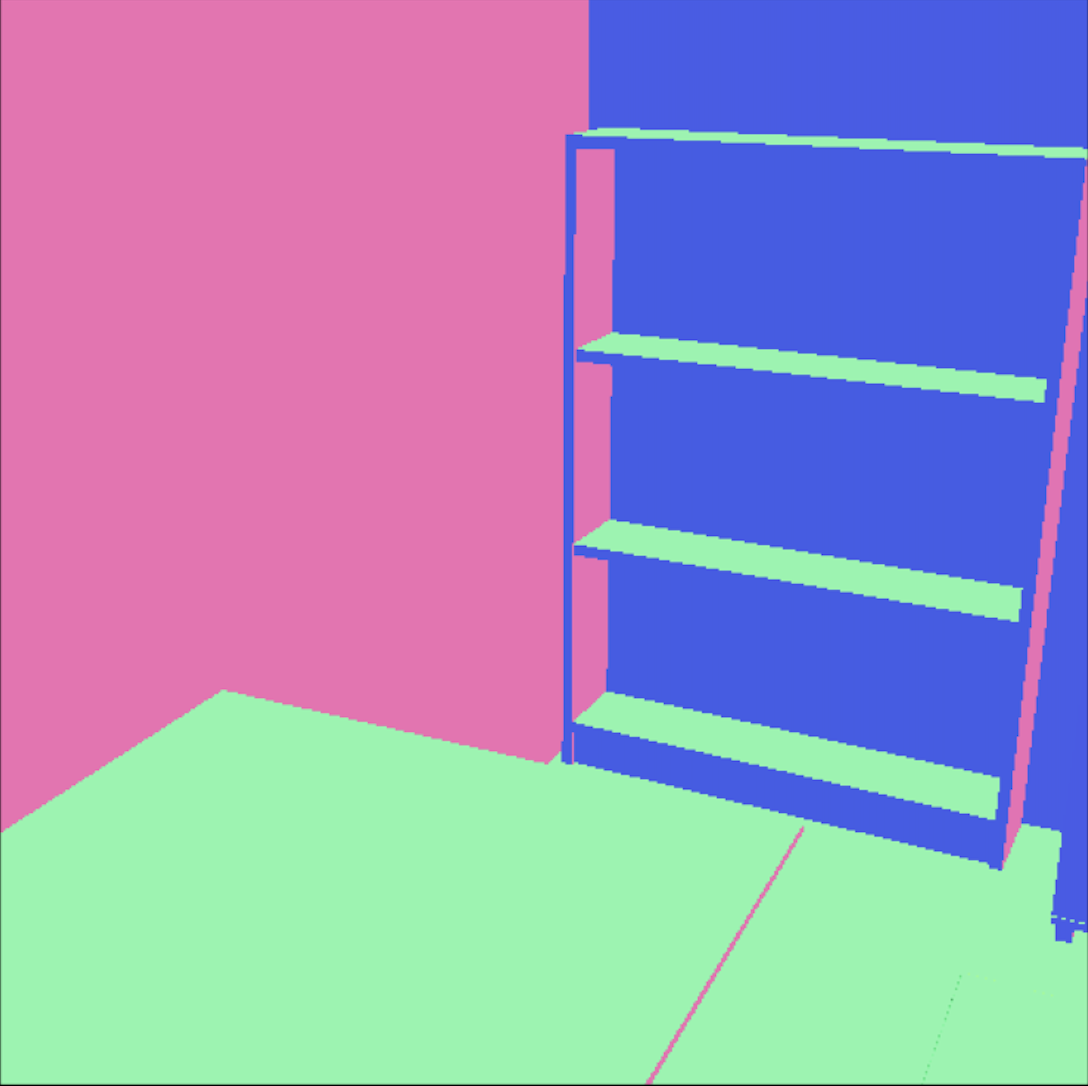
\includegraphics[width=.2\linewidth,valign=m]{/Users/apple/OVGU/Thesis/code/3dReconstruction/report/images/realistic_images_relatedwork/blenderproc_normal_1}\\


        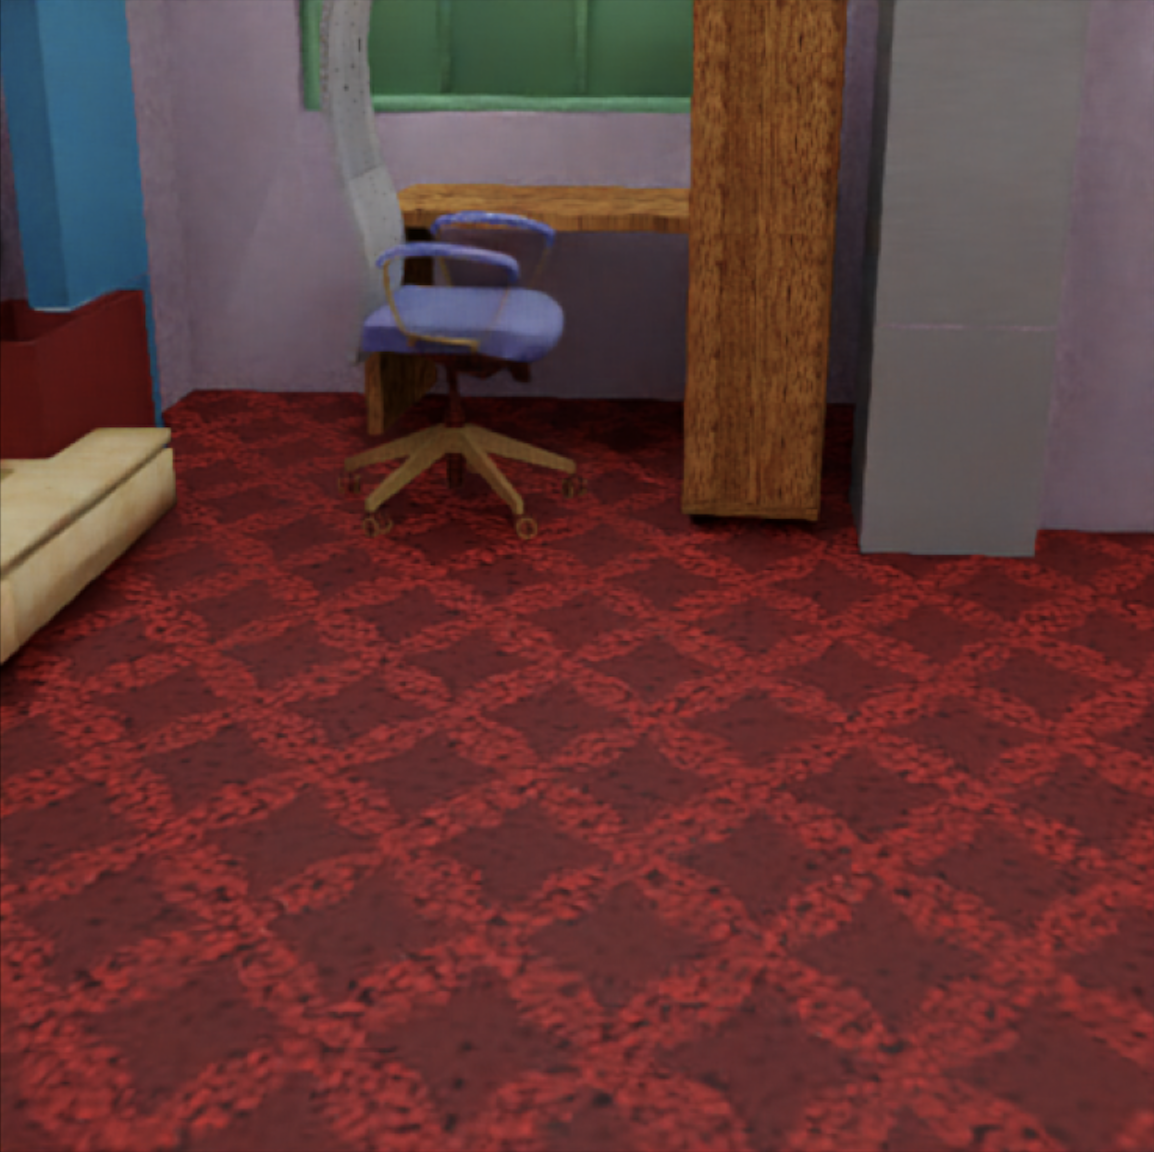
\includegraphics[width=.2\linewidth,valign=m]{/Users/apple/OVGU/Thesis/code/3dReconstruction/report/images/realistic_images_relatedwork/blenderproc_2} &
        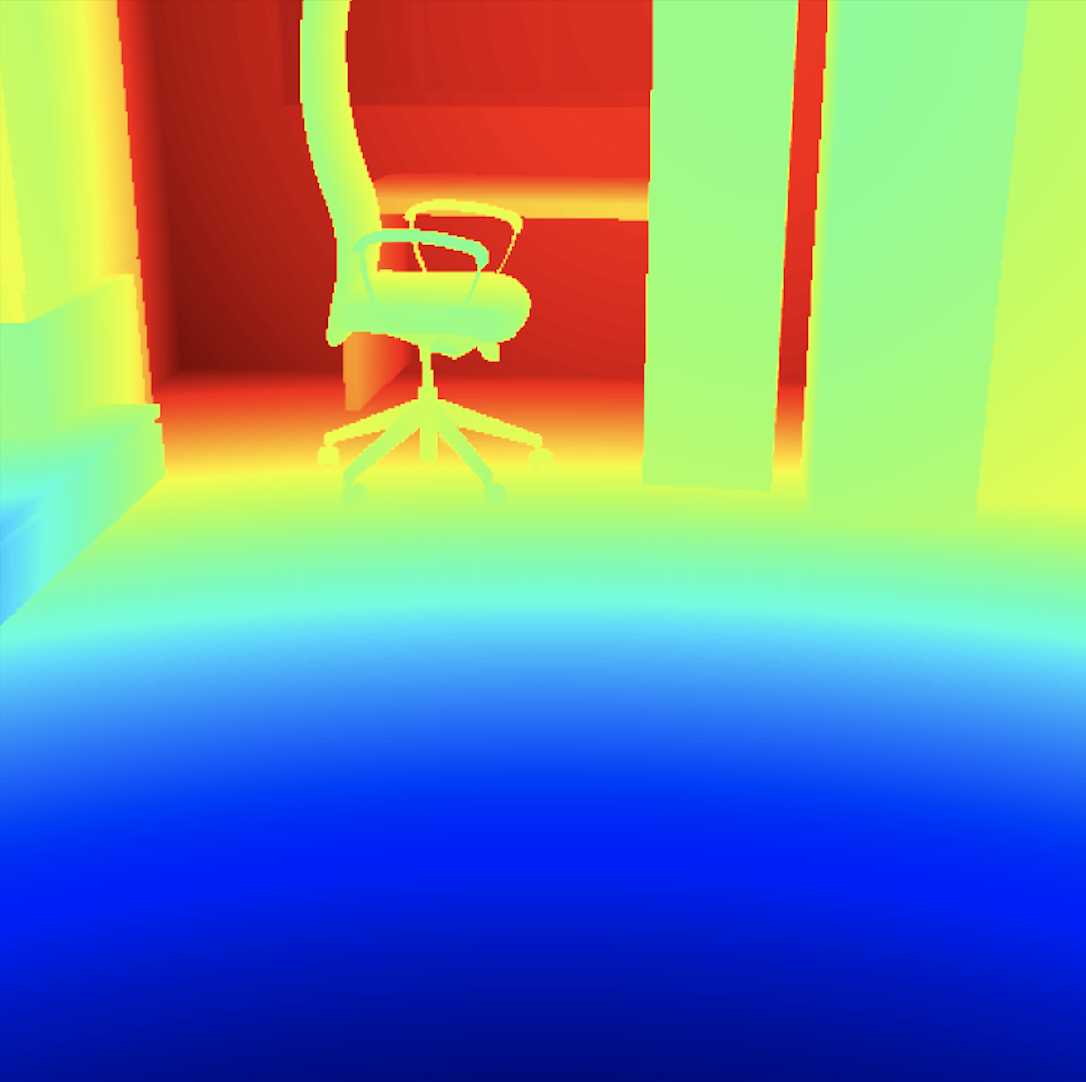
\includegraphics[width=.2\linewidth,valign=m]{/Users/apple/OVGU/Thesis/code/3dReconstruction/report/images/realistic_images_relatedwork/blenderproc_depth_2} &
        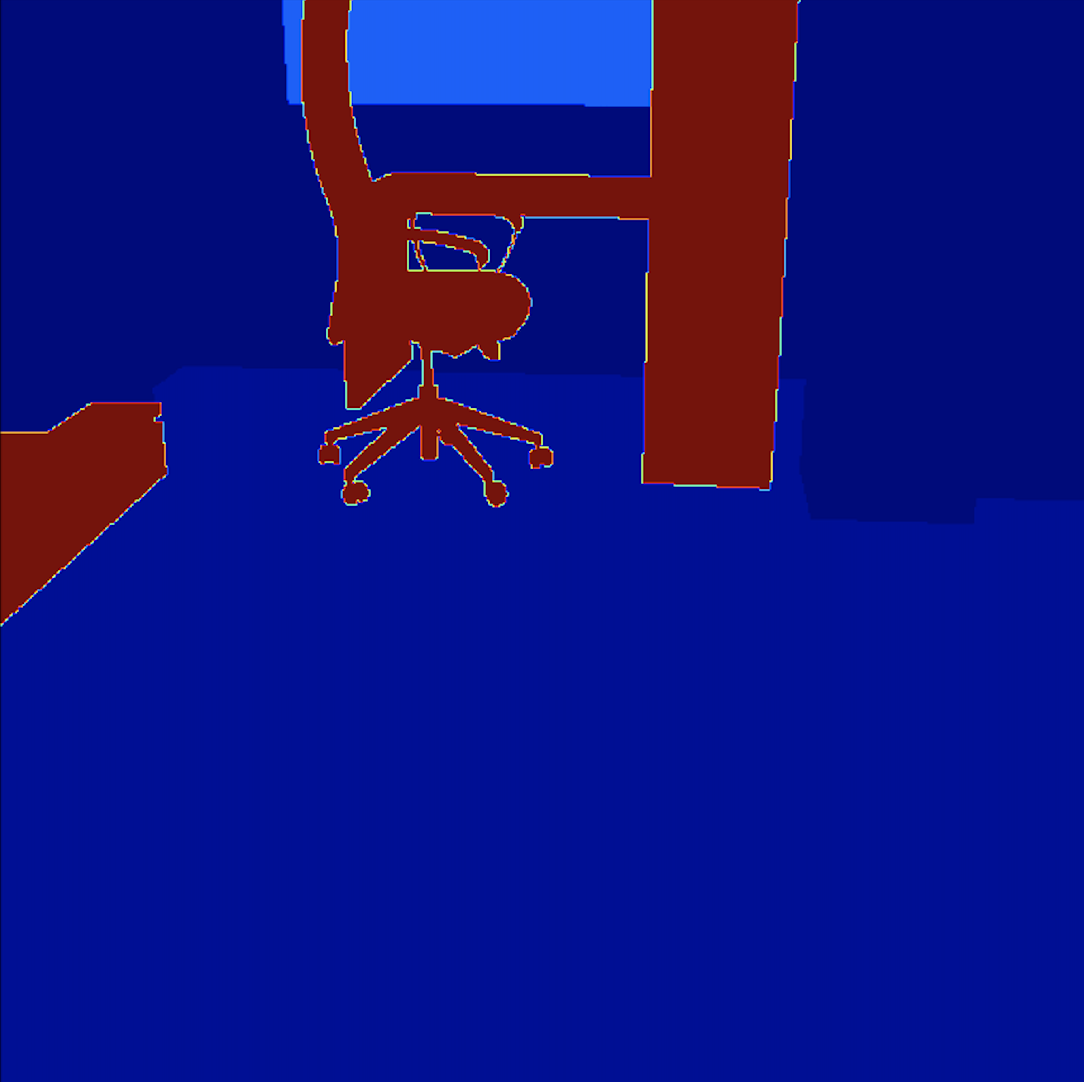
\includegraphics[width=.2\linewidth,valign=m]{/Users/apple/OVGU/Thesis/code/3dReconstruction/report/images/realistic_images_relatedwork/blenderproc_instance_2} &
        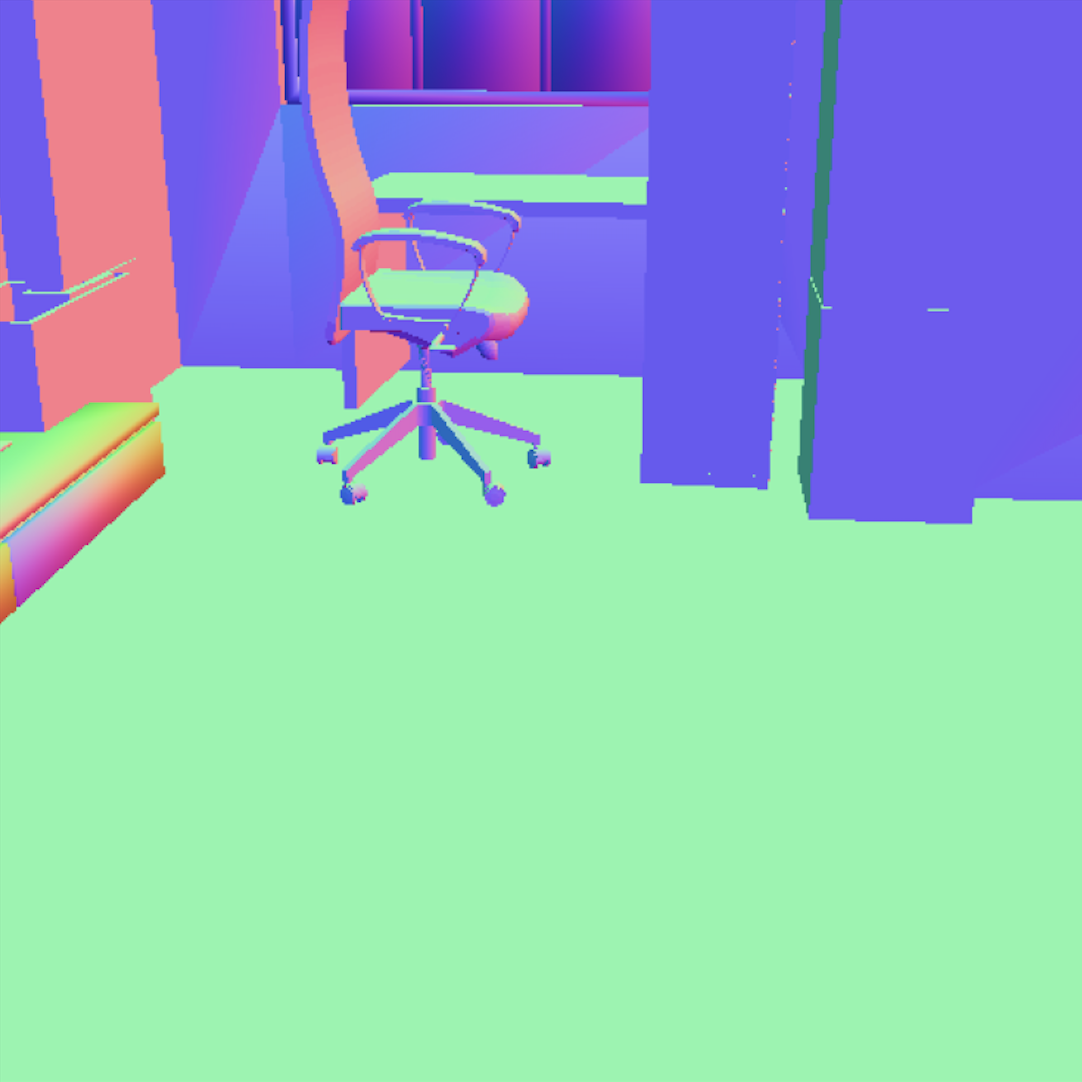
\includegraphics[width=.2\linewidth,valign=m]{/Users/apple/OVGU/Thesis/code/3dReconstruction/report/images/realistic_images_relatedwork/blenderproc_normal_2}\\

%        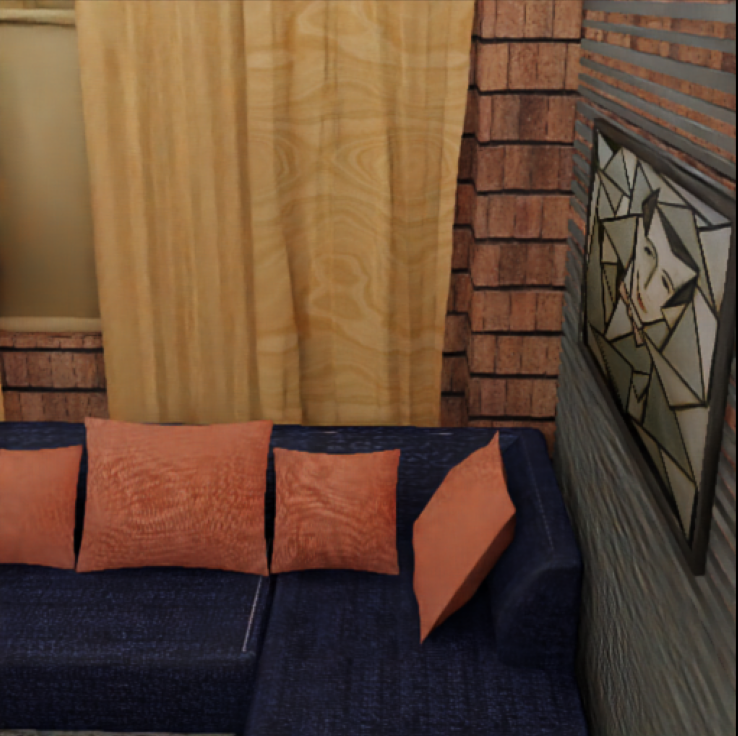
\includegraphics[width=.2\linewidth,valign=m]{/Users/apple/OVGU/Thesis/code/3dReconstruction/report/images/realistic_images_relatedwork/blenderproc_3} &
%        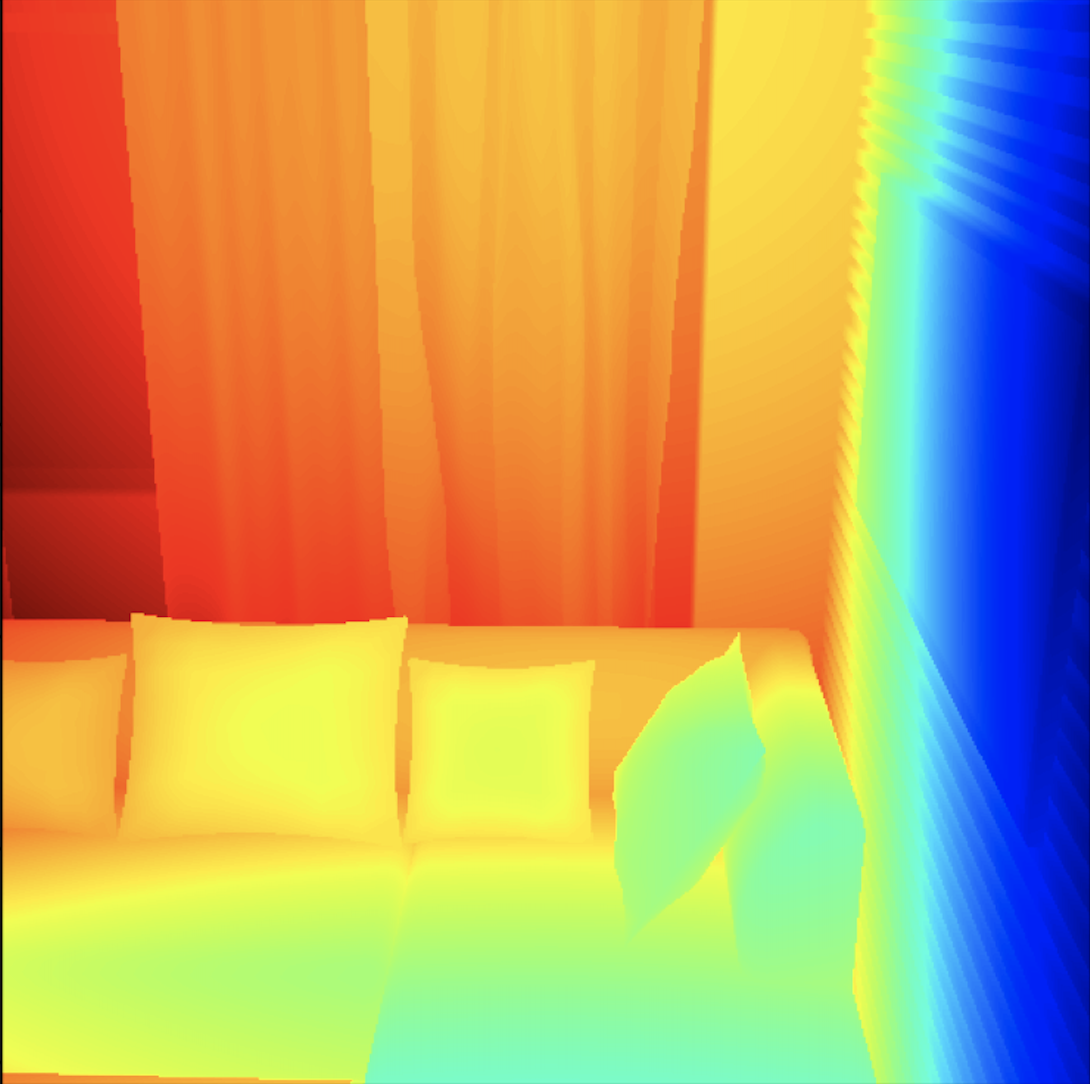
\includegraphics[width=.2\linewidth,valign=m]{/Users/apple/OVGU/Thesis/code/3dReconstruction/report/images/realistic_images_relatedwork/blenderproc_depth_3} &
%        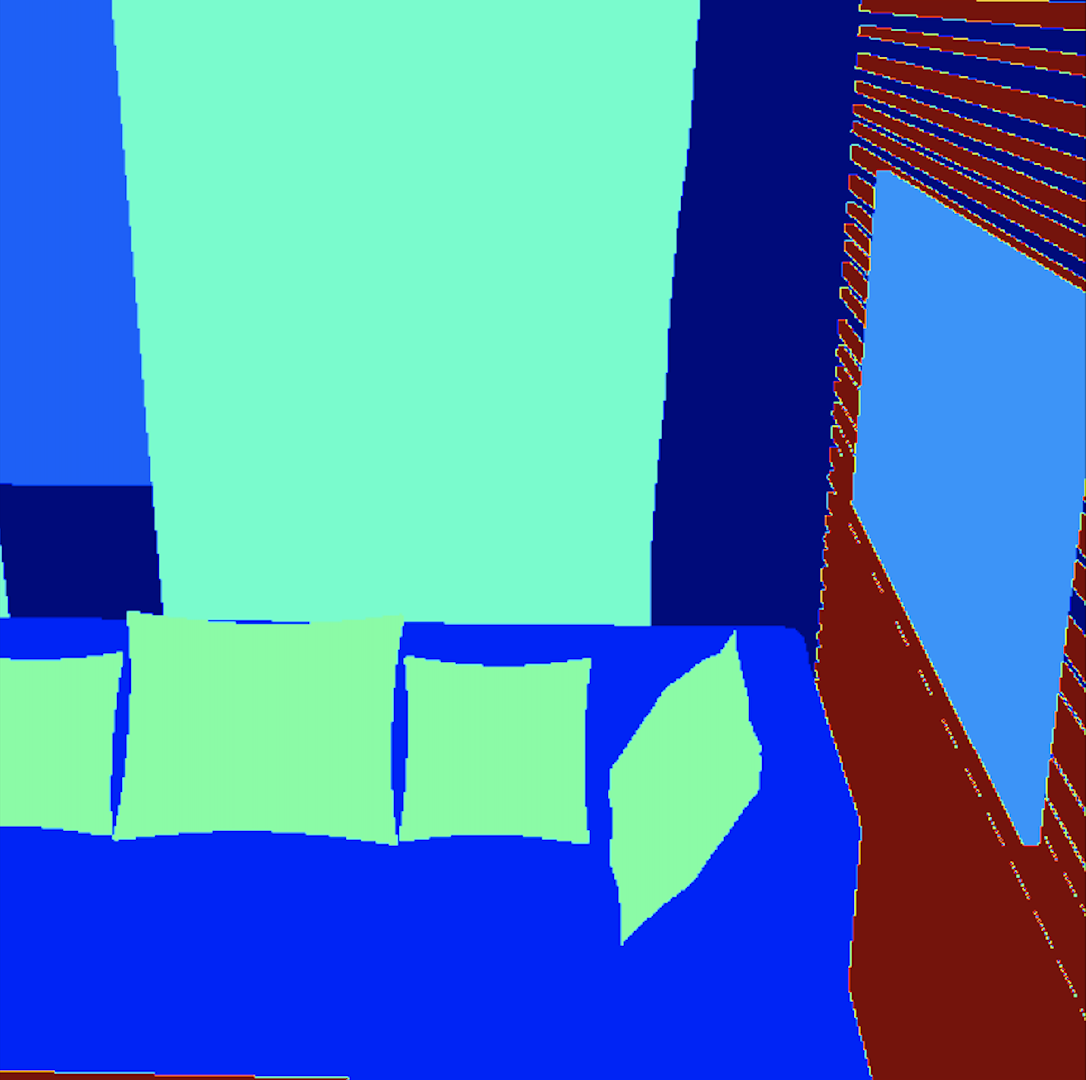
\includegraphics[width=.2\linewidth,valign=m]{/Users/apple/OVGU/Thesis/code/3dReconstruction/report/images/realistic_images_relatedwork/blenderproc_instance_3} &
%        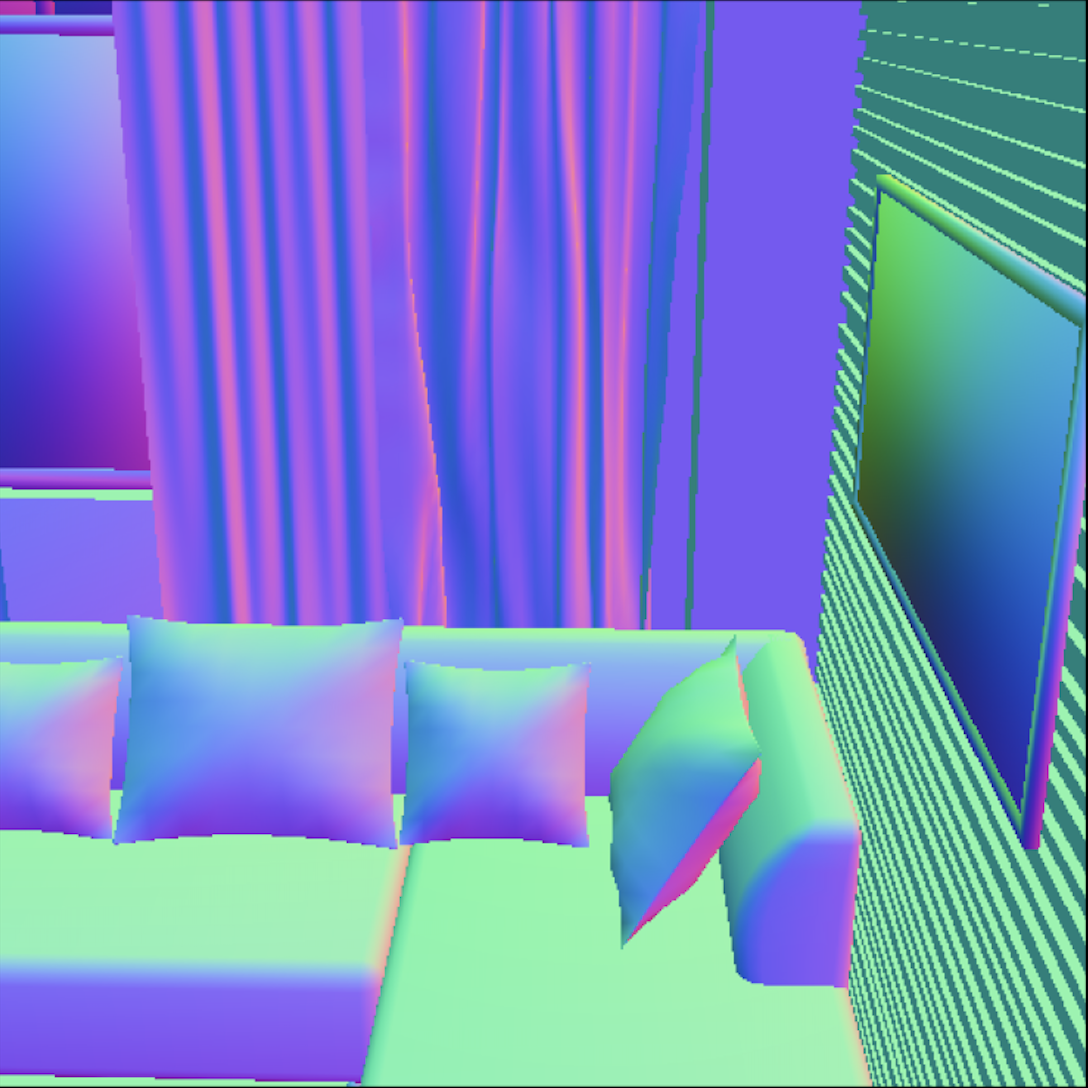
\includegraphics[width=.2\linewidth,valign=m]{/Users/apple/OVGU/Thesis/code/3dReconstruction/report/images/realistic_images_relatedwork/blenderproc_normal_3}\\

    \end{tabular}
    \caption{Sample images created from BlenderProc using SceneNet dataset.(Left to right) RGB images, Depth Maps, Instance Segmenatations and Normals. Each row is an independent sample.}
    \label{fig:Blenderproc samples}
\end{figure}

NVIDIA developed a Deep learning Dataset Synthesizer (NDDS)~\cite{to2018ndds} in the form of a plugin for Unreal Engine 4(UE4).
The plugin can synthesize images, per-pixel segmentation, depth, object 3D pose, 2D/3D bounding box, keypoints, and custom stencils.
It even supports domain randomization of objects, lighting, camera position, poses, and textures.
They Leveraged the asynchronous, multithreaded frames to generate data at high rates(50-100 Hz) for Falling Things (FAT)~\cite{Tremblay2018} dataset.

``SynthDet: An end-to-end object detection pipeline using synthetic data"~\cite{synthdet2020} is an open-source project supported by Unity technologies using Unity Engine.
This ML pipeline uses 63 everyday objects(example: cereal box, cady, cartons, and more) as synthetic objects to generate 2D bounding boxes.
This project was highly influenced by~\cite{hinterstoisser2019annotation}, wherein they used synthetic 3D models with a randomized background to generate a synthetic dataset for the object detection task.
With domain randomization, the author of~\cite{hinterstoisser2019annotation} proved that no real data or mixed training is required for the Deep Learning model to perform significantly.

UnrealCV~\cite{Qiu2017} is an open-source project built upon Unreal Engine 4 (UE4)\footnote{Epic Games, Unreal Engine:https://www.unrealengine.com}).
It supports some pre-built indoor architectures available on the asset store, which are unfortunately paid versions.
Along with this limitation, the plugin only creates depth maps, normals, and segmentation masks, with no mapping to 3D models.
Another tool based on the Unreal engine is UnrealROX+\cite{martinezgonzalez2021unrealrox}.
This plugin design is based on UnrealCV and provides similar data.

\section{Domain space}\label{sec:domain-space}

Since this thesis includes image datasets from different domains, it is essential to understand the domain space of these datasets.
When two or more datasets originate from different sources we say the datasets belong to different domains.
Synthetic and Real datasets are collected or generated using different methods, and hence they have a different domain space.
This section discusses how we intend to visualize the domain space and a quantitative measure to indicate the difference between the domains.

\subsection{Visualizing with \gls{tsne}}\label{subsec:visualizing-with-tsne}
\gls{tsne} stands for t-Distributed Stochastic Neighbor Embedding~\cite{vanDerMaaten2008}; it is a tool to visualize a high dimensional space in a low dimension space while retaining the information of high dimension as much as possible.
In our case, the images are embedded using a \gls{vgg}16 network with an output dimension of 1000.
This multi-dimensional output is converted to two-dimension for better visualization of the embedding space.

In this segment, we briefly explain how \gls{tsne} works.

\begin{enumerate}
    \item \textbf{Step 1}: Calculate the similarity between points in high dimensional space using a joint probability distribution.
    To achieve this, the Euclidean distances between each point is transformed into conditional probability distribution as in \autoref{eq:equation1}, which represents similarity between a pair of points.
    The conditional probability of a point $x_i$ with point $x_j$ to be located next to it, is represented by a Gaussian with center at $x_i$.
    Normalising is done to handle the different cluster densities.
    Conditional probability is converted to Joint probability using \autoref{eq:equation2}.
    \begin{equation}
        p_{j \mid i}=\frac{\exp \left(-\left\|x_{i}-x_{j}\right\|^{2} / 2 \sigma_{i}^{2}\right)}{\sum_{k \neq i} \exp \left(-\left\|x_{i}-x_{k}\right\|^{2} / 2 \sigma_{i}^{2}\right)}
        \label{eq:equation1}
    \end{equation}

    \begin{equation}
        p_{i j}=\frac{p_{j \mid i}+p_{i \mid j}}{2 n}
        \label{eq:equation2}
    \end{equation}

    \item \textbf{Step 2}: Using a random point dataset on a lower dimension with same number of points in higher dimension, a Joint probability distribution is created but with a Student-t distribution instead of Gaussian.
    This is represented by \autoref{eq:equation3}.
    t-distribution makes sure that the projection in low dimension is not concentrated on a single point.
    \begin{equation}
        q_{ij} = \frac{(1+\left \| y_{i}-y_{j} \right \|^{2})^{-1}}{\sum _{k\neq l} (1+\left \| y_{k}-y_{l} \right \|^{2})^{-1}}
        \label{eq:equation3}
    \end{equation}

    \item \textbf{Step 3}: Learn to represent the high dimension space in low dimension by making the Joint distribution of the lower dimension as close as possible to that of the higher dimension.
    For this Kullback-Leiber divergence\cite{Joyce2011} is used to compare the similarity between the two distributions as in \autoref{eq:equation4}.
    Using gradient descent, the cost function based on KL-divergence (\autoref{eq:equation5}) is minimized to make the points fall in place.

    \begin{equation}
        D_{\mathrm{KL}}(P \| Q)=\sum_{x \in \mathcal{X}} P(x) \log \left(\frac{P(x)}{Q(x)}\right)
        \label{eq:equation4}
    \end{equation}

    \begin{equation}
        C=K L(P \| Q)=\sum_{i} \sum_{j} p_{i j} \log \frac{p_{i j}}{q_{i j}}
        \label{eq:equation5}
    \end{equation}
\end{enumerate}

Perplexity is a parameter that informs the algorithm on how much attention to give the local and global features.
The publication~\cite{vanDerMaaten2008} indicates the values between 5 and 50 to be a good initialization.
An article on \gls{tsne} interpretation~\cite{wattenberg2016how} informs us to have a perplexity value lesser than the total number of points.
It also notes that the cluster distance may not be as the intuition suggests, i.e., greater distance may not necessarily mean good separation, or lesser distance does not inevitably mean closer similarity for well-separated clusters.
However, \gls{tsne} can still visualize if the clusters are overlapping or have a shared embedding space or not.
Hence, we will use \gls{tsne} as a medium to visualize the embedding space without giving importance to the distance or the scale of the plots.

%\subsection{Maximum Mean Discrepancy(MMD)}
\subsection{Fr\'echet Inception Distance(FID))}\label{subsec:fr'echet-inception-distance)}
For quantitative measure, we use \gls{fid}
\gls{fid} \cite{Heusel2017GANsTB} was specifically formulated to evaluate the performance of Generative Adversarial Networks \cite{Goodfellow2014}.
The core idea behind \gls{fid} was to evaluate the generated synthetic images using the statistics collected from both synthetic and real images.
Lower the value of \gls{fid} better the quality of the images.

The embeddings of the images are calculated by passing it through an Inception v3 model~\cite{Szegedy2016RethinkingTI} pre-trained on ImageNet~\cite{Deng2009ImageNetAL}.
The output layer is removed, and the penultimate pooling layer activations are used to get the embedding vector.
This vector has a dimension of 2048.
The images from both synthetic and real datasets are passed through the model, and the obtained statistics is used to calculated the \gls{fid} as in \autoref{eq:fid}.

\begin{equation}
    d^{2}\left((\boldsymbol{\mu}_{r}, \boldsymbol{C}_{r}),\left(\boldsymbol{\mu}_{s}, \boldsymbol{C}_{s}\right)\right)=\left\|\boldsymbol{\mu}_{r}-\boldsymbol{\mu}_{s}\right\|^{2}+\operatorname{Tr}\left(\boldsymbol{C}_{r}+\boldsymbol{C}_{s}-2\left(\boldsymbol{C}_{w} {C}_{w}\right)^{1 / 2}\right)
    \label{eq:fid}
\end{equation}

In the above \autoref{eq:fid}, $\mu_r$ and $\mu_s$ are feature-wise mean for real and synthetic images, $C_r$ and $C_s$ are respective covariance matrices.
$Tr$ is the Trace linear algebra operation, which is the sum of main diagonal elements.


\section{Mitigating domain shift}\label{sec:mitigating_domain_shift}

The idea of domain randomization is that real images appear to be one of the many variations among training images from synthetic datasets.
Thus, testing with real-world images should give a comparable performance.
~\cite{tobin2017domain} used this principle for small objects detection tasks used for robotics.
This paper tries different parameters in domain randomization like lights, camera viewpoints, and textures and combines domain randomization with domain adaptation.

~\cite{prakash2020structured} introduced Structured domain randomization, where the structure and context are preserved for the problem while creating synthetic images.
Example: A road is randomly placed with parameters like curvature, lighting, and camera position.
With this as context, they generate pedestrian walk, road lanes, etc.
After these two steps, the objects such as cars, cyclists, houses, buildings are placed on the scene.
As an ablation study, the author changes domain randomization parameters and checks the performance of the car detection task.

~\cite{georgakis2017synthesizing} proposed domain randomization-based synthetic images generation to detect objects found in the kitchen.
The objects are cropped and placed on the background with semantic information and geometry with proper scale.
Similar to the above works, the author also provides an ablation study with different ratios of synthetic to the real dataset for mixed training.

Domain randomization and adaptation techniques are not the only ways to mitigate the domain shift.
With the advent of Generative Adversarial Networks~\cite{Goodfellow2014}, synthetic to real image conversions have become possible and lead to better performance on given tasks.
~\cite{Richter_2021, CycleGAN2017, park2020cut,isola2017image, dundar2018domain,Wang2018HighResolutionIS} are some successful attempts to reduce the gap between simulated environment and reality.
Intel in~\cite{Richter_2021} uses the GTA V dataset with G-buffers(depth, normals, segmentations, Albedo, glossiness, etc.) to enhance the photorealism of synthetic images.
~\cite{park2020cut} use a patchwise contrastive loss to retrain the content of the input image.
They minimize the loss such that corresponding patches retain high mutual values.

Another exciting way to reduce the domain gap is using domain adversarial training~\cite{Ganin2017}.
Along with the task under observation, a branched network from the feature extractor is used as a classifier for the domains.
This acts like a multi-learning task where the feature extractor is the common branch.
In one branch, the model learns to perform a specific task like segmentation or classification.
The other branch classifies if the dataset is real or synthetic.
~\cite{Pinheiro2019} implement the same principle on complex 3D reconstruction tasks by predicting voxels and classifying the image domain.

\subsection{Training with synthetic dataset}\label{subsec:training-with-synthetic-dataset}
The research questions, as stated in \autoref{sec:goal} aims to check if a synthetic dataset can deliver as a standalone dataset.
If it does not, then techniques like fine-tuning will be helpful.
Another way to use the large synthetic datasets is using mixed training.

In~\cite{nowruzi2019real},  the author tries to find how much real data is required with the synthetic dataset to increase the performance of object detection tasks.
A study was conducted by training various object detection models on mixed data containing different real and synthetic datasets ratios.
The four ratios considered for mixed training were 0\%, 90\%, 95\%, 97.5\% of synthetic data to real data.
Another study was conducted by fine-tuning a model pre-trained on a synthetic dataset with real datasets of different sizes.
They observed that fine-tuning with a limited real dataset is better than mixed training with a synthetic dataset.

~\cite{Tremblay2018TrainingDN}  explore domain randomization on real-world object detection.
The author also proposes a new approach of domain randomization, wherein random 3d objects called ”flying distractors” are randomly placed in the scene;
the model learns to ignore objects that are not of interest.
A focused ablation study with individual domain randomization parameters was also conducted to understand the contribution of each component.
The parameters included lights, textures, data augmentation, and flying distractor, as mentioned above.
Also, object detection is trained with varying dataset sizes to learn its impact.
They also conducted a study of the dataset size needed to fine-tune a pre-trained model optimally.

\cite{synthia} is a synthetic dataset for semantic segmentation of urban scenes with 13 classes.
In this paper, the author combines the proposed synthetic dataset and the real dataset from~\cite{Geiger2012CVPR,Russell2008,BrostowSFC:ECCV08} to show boost in performance of semantic segmentation task.
The mixing ratio is 60\% per min-batch.
The author also notes that only 33\% of real dataset was required with combination of synthetic dataset to get a performance equivalent to model trained on only real dataset.

